% !TeX root=../main.tex
\chapter{پیاده‌سازی}

% ------------ Section 4.1
\section{نوشتن کد قرارداد}
در این بخش به بررسی مراحل و نحوه نوشته شدن کد قرارداد هوشمند پرداخته می‌شود.

% ------------ Sub Section 4.1.1
\subsection{نیازمندی‌های قرارداد هوشمند}
نیازمندی‌های اصلی کاپو به ترتیب زیر است.
\begin{itemize}
  \item
هر آدرس در شبکه بتواند یک داده‌ی متنی را به آسان‌ترین و کم هزینه‌ترین روش ممکن به یک توکن تعویض‌ناپذیر تبدیل کند.
  \item
هر آدرس بتواند توکن‌های خود را به اشخاص دیگر انتقال دهد و یا در بازارهای معاملات توکن‌های تعویض‌ناپذیر بفروشد.
  \item
در صفحه اول وبسایت تعداد کل توکن‌های ساخته شده تا به حال و تعداد کل صاحبان توکن‌ها نمایش داده شود.
  \item
قابلیت‌های قرارداد هوشمند تست شده باشد.
\end{itemize}

% ------------ Sub Section 4.1.2
\subsection{ارث‌بری}
با توجه به مزایای ذکر شده در مورد استانداردسازی قراردادهای هوشمند،
انتخاب درست این است که برای پیاده‌سازی این کاربری از یکی از استانداردها استفاده شود.
\gls{Inheritance}
از استانداردهای یک کتابخانه متن‌باز مزایای زیر را فراهم می‌کند.
\begin{itemize}
  \item
به دلیل وجود کدهای پایه به صورت آماده سرعت توسعه پروژه افزایش می‌یابد.
  \item
ارتباط دیگر پروژه‌ها با پروژه کاپو به راحتی انجام می‌شود.
  \item
امنیت قرارداد و درستی آن حداقل در سطوح پایه‌ای تا حد خوبی تضمین شده است.
\end{itemize}

قرارداد هوشمند کاپو از استاندارد
\lr{ERC721}
پیاده‌سازی شده در کتابخانه اپن‌زپلین
\LTRfootnote{
  \url{https://github.com/OpenZeppelin/openzeppelin-contracts}
}
ارث‌بری می‌کند که یکی از معروف ترین کتابخانه‌های پیاده کننده استانداردهای قرارداد هوشمند است.

% ------------ Sub Section 4.1.3
\subsection{توجه به هزینه تراکنش و نوع توابع}
در نوشتن یک قرارداد هوشمند باید به نکات زیر توجه کنیم.
\begin{itemize}
  \item
میزان حافظه‌ای که توسط داده‌های قرارداد روی شبکه بلاکچین اشغال می‌شود.
  \item
حجم بایت‌کد قرارداد هوشمند.
  \item
تعداد عملیات‌های هر متد، به خصوص متدهایی که مکررا مورد استفاده کاربر قرار می‌گیرند.
  \item
نوع هر متد، که مشخص می‌کند هر متد تا چه حد روی شبکه بلاکچین تغییر ایجاد می‌کند.
\end{itemize}

توجه نکردن به هریک از این موضوعات باعث می‌شود که قرارداد هوشمند به اندازه کافی بهینه عمل نکند و کاربر وادار به پرداخت
\gls{Gas fee}
بیشتر شود.
یکی از مهمترین نکاتی که برای بهینه‌تر رفتار کردن قرارداد هوشمند
باید به آن توجه کنیم نوع هر متد است.

اگر متدی از نوع
\lr{pure}
تعریف شود به این معنی است که به هیچ اطلاعاتی از شبکه بلاکچین نیاز ندارد
و همه‌ی اطلاعاتی که لازم دارد را در اسکوپ
\LTRfootnote{Scope}
خودش دارد. اگر متدی از نوع
\lr{view}
باشد به این معنی است که به اطلاعاتش روی شبکه بلاکچین نیاز دارد
اما فقط می‌خواهد آن‌ها را بخواند و نمیخواهد تغییری در آن‌ها ایجاد کند.
این دو نوع متد نیازی به پرداخت کارمزد تراکنش توسط کاربر ندارند.
اما اگر در تعریف متدی ذکر نشود که یکی از این دو نوع است، اینطور در نظر گرفته می‌شود
که نیاز به بروزرسانی اطلاعاتش در شبکه بلاکچین دارد
و از کاربری که آن را فراخوانی کرده است هزینه تراکنش بیشتر دریافت می‌شود.


% ------------ Sub Section 4.1.4
\subsection{جزئیات فنی پیاده‌سازی}
ساخت توکن‌های تعویض‌ناپذیر در این قرارداد به آدرس‌های مشخص محدود نیست و همه می‌توانند توکن بسازند.
بسیاری از قراردادها برای صرفه‌جویی در هزینه تراکنش کاربران اکثر اطلاعات مربوط به توکن‌ها را در قرارداد نگه نمی‌دارند
و فقط داده‌های بسیار مهم توکن مانند شناسه آن را در شبکه بلاکچین نگهداری می کنند.
از آنجایی که کاپو یک قرارداد همه منظوره است و ممکن است استفاده‌های فراوانی داشته باشد،
تصمیم‌گیری این مورد به عهده کاربر قرارداد گذاشته می‌شود.

در کاپو شناسه هر توکن از
\gls{Hash}
داده‌های توکن به دست می‌آید.
این نحوه عملکرد یک مزیت بسیار مهم ایجاد می‌کند،
به این ترتیب هیچ دو توکنی نمی‌توانند داده‌های یکسان داشته باشند،
زیرا در این صورت شناسه آن‌ها باید یکسان باشد و این امکان پذیر نیست زیرا شناسه توکن‌ها یکتاست.

در یک قرارداد
\lr{ERC721}
استاندارد فقط شناسه توکن‌ها ذخیره می‌شود. در کاپو علاوه بر شناسه توکن‌ها یک
\gls{Mapping}
از شناسه توکن‌ها به داده‌ی آن‌ها با نام
\lr{tokenDatas}
نیز نگهداری می‌شود. همچنین در کاپو نگاشت دیگری نیز از آدرس به لیست توکن‌های آن آدرس با نام
\lr{ownerTokens}
نگهداری می‌شود.
متغیر اول کمک می‌کند که با داشتن شناسه یک توکن به راحتی داده آن توکن به دست آورده شود.
متغیر دوم نیز کمک می‌کند که به راحتی بتوان توکن‌های یک آدرس را به دست آورد. دو متغیر دیگر با نام‌های
\lr{numberOfTokenHolders}
و
\lr{numberOfMintedTokens}
نیز در کاپو نگه‌داشته می‌شوند که برای نمایش آمار استفاده از قرارداد در صفحه اصلی اپلیکیشن مورد استفاده قرار می‌گیرند.

متد
\lr{mint}
به نحوی نوشته شده است که برای عموم قابل استفاده باشد.
پس از محاسبه هش داده‌ی توکن از آن به عنوان شناسه توکن استفاده می‌شود،
توکن ساخته می‌شود و متغیرهای
\lr{tokenDatas}
و
\lr{numberOfMintedTokens}
بروزرسانی می‌گردند.
پیاده‌سازی این متد را می‌توان در تصویر
\ref{fig:mint}
مشاهده کرد.

\begin{figure}
\centerline{\frame{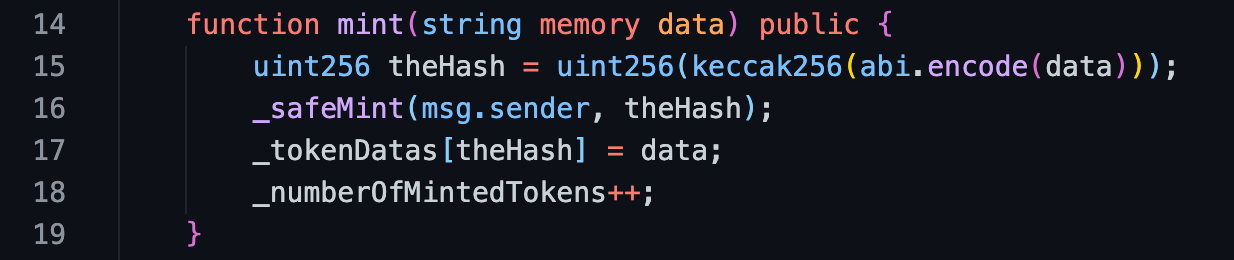
\includegraphics[width=12cm]{mint.png}}}
\caption{پیاده‌سازی تابع mint}
\label{fig:mint}
\end{figure}

متد
\lr{afterTokenTransfer}
از استاندارد
\lr{ERC721}
به نحوی بازنویسی
\LTRfootnote{Overwrite}
شده است که پس از هر انتقال توکن با بررسی آدرس‌های مبدا و مقصد، متغیر‌های
\lr{numberOfTokenHolders}
و
\lr{numberOfMintedTokens}
و
\lr{ownerTokens}
را بروزرسانی کند.
نحوه عملکرد این متد در تصویر
\ref{fig:afterTokenTransfer}
مشخص است.

\begin{figure}
\centerline{\frame{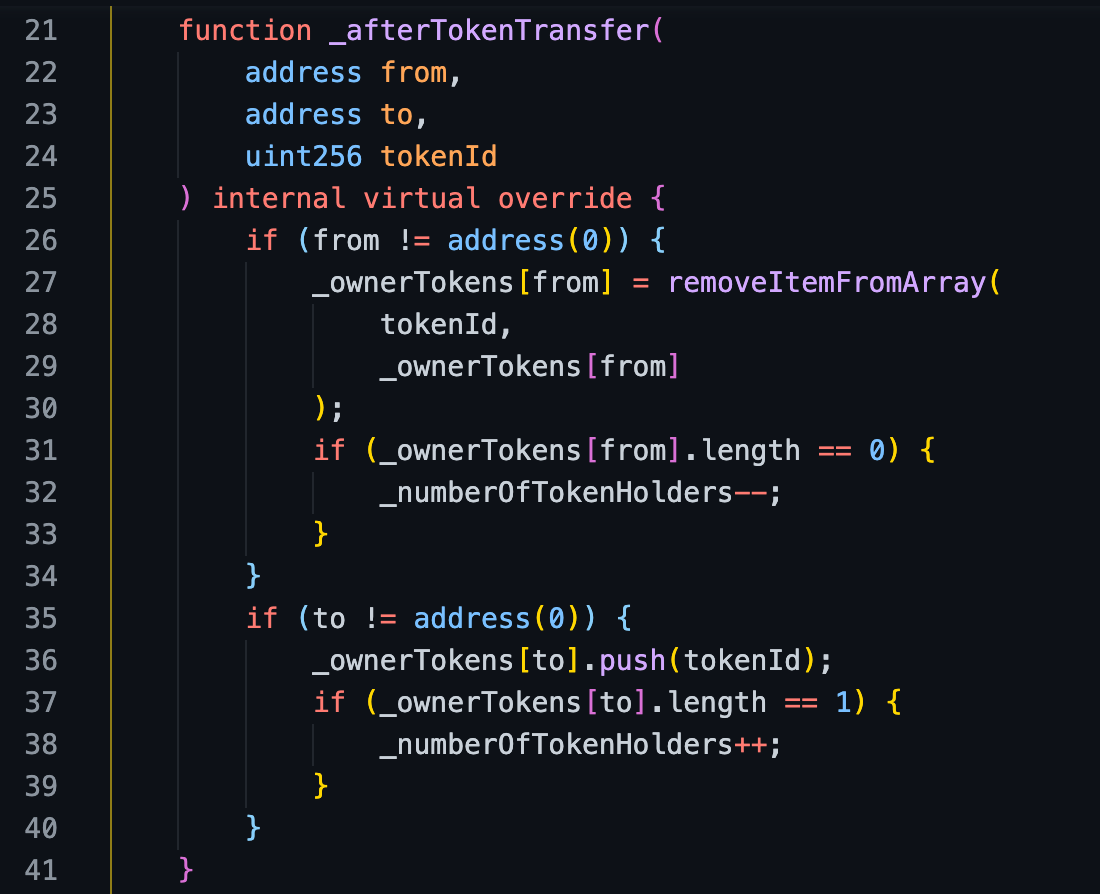
\includegraphics[width=12cm]{afterTokenTransfer.png}}}
\caption{پیاده‌سازی تابع afterTokenTransfer}
\label{fig:afterTokenTransfer}
\end{figure}

متد جدیدی با نام
\lr{getUserTokens}
نیز نوشته شده است که در استاندارد
\lr{ERC721}
به صورت پیش‌فرض وجود ندارد. این متد با گرفتن یک آدرس و استفاده از
\lr{ownerTokens}
و
\lr{tokenDatas}
دو خروجی برمی‌گرداند، لیستی از شناسه توکن‌های آدرس و لیستی از داده‌های توکن‌های آدرس.
محتوای این متد در تصویر
\ref{fig:getUserTokens}
قابل مشاهده است.

\begin{figure}
\centerline{\frame{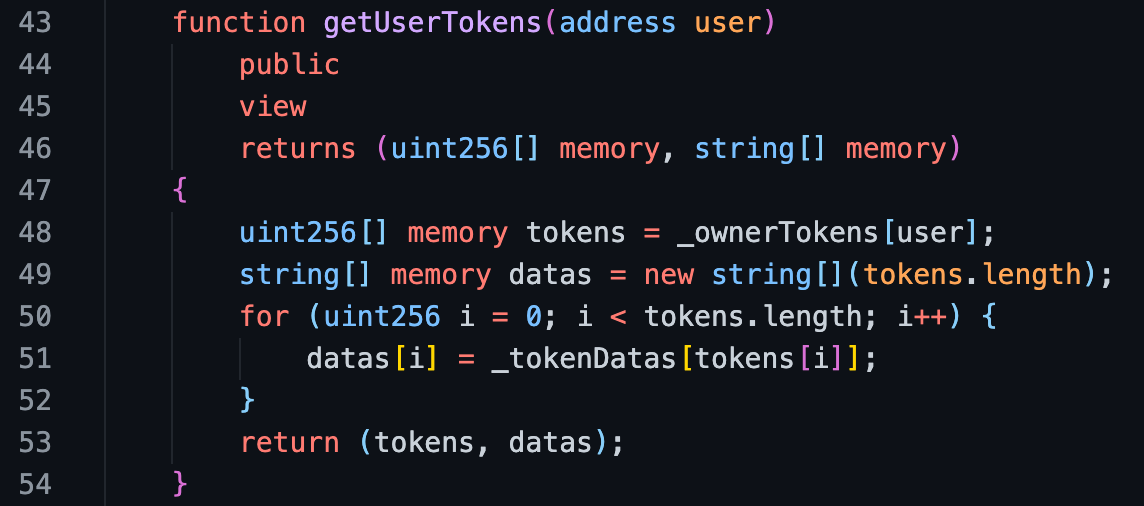
\includegraphics[width=12cm]{getUserTokens.png}}}
\caption{پیاده‌سازی تابع getUserTokens}
\label{fig:getUserTokens}
\end{figure}

زبان سالیدیتی به طور پیش‌فرض امکان حذف یک داده از یک آرایه با داشتن مقدار آن را ندارد.
دلیل عدم وجود این قابلیت هزینه‌بر بودن آن است.
در سالیدیتی توسعه دهندگان به استفاده از
\gls{Mapping}
و دوری از آرایه‌ها تشویق می‌شوند.
اما برای نمایش نحوه ارث‌بری از بیش از یک قرارداد پدر، برای کاپو یک قرارداد به نام
\lr{Helper}
نوشته شد که قابلیت حذف کردن یکی از اعضای آرایه با داشتن مقدارش را فراهم می‌کند.
این قرارداد در تصویر
\ref{fig:Helper}
قابل مشاهده است. کاپو علاوه بر
\lr{ERC721}
از قرارداد Helper نیز ارث‌بری می‌کند.

\begin{figure}
\centerline{\frame{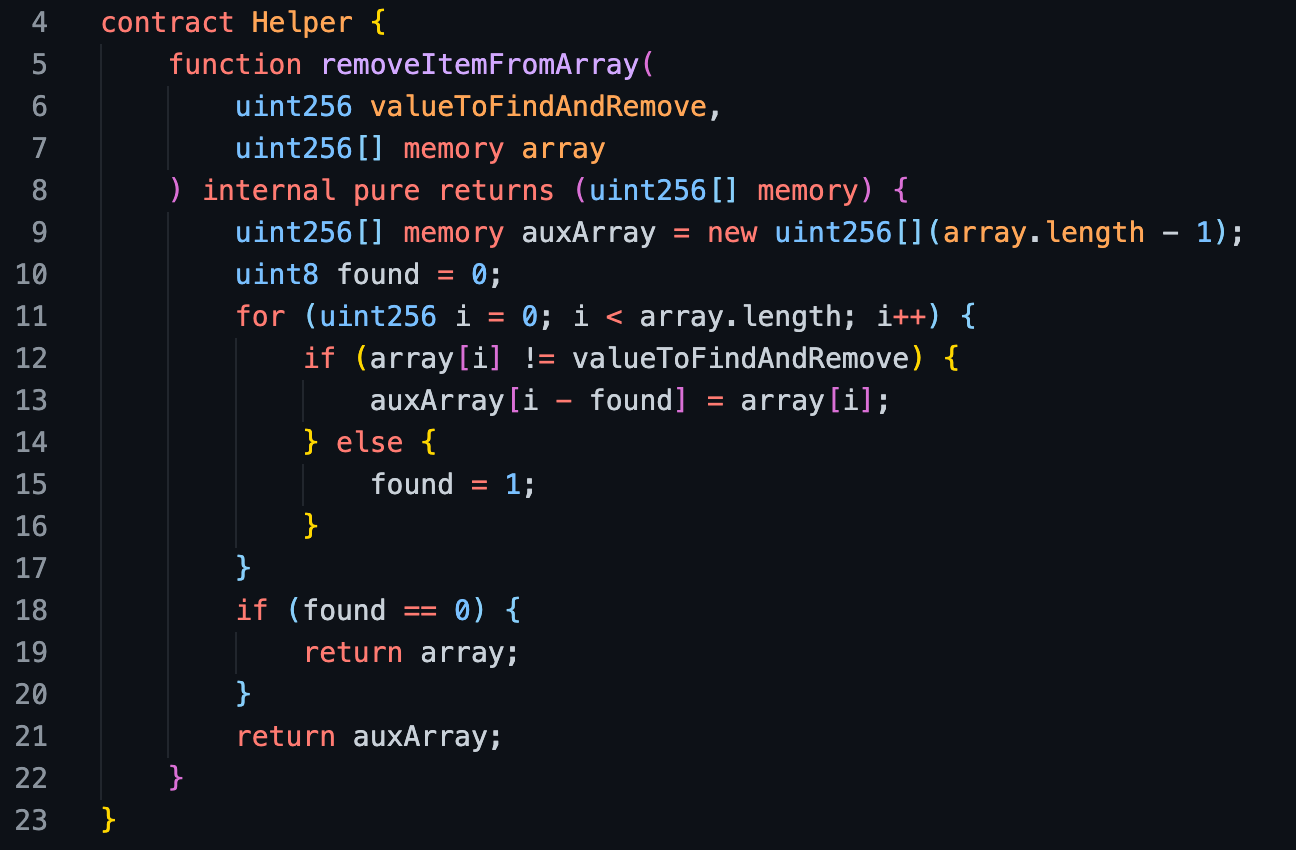
\includegraphics[width=12cm]{Helper.png}}}
\caption{پیاده‌سازی قرارداد Helper}
\label{fig:Helper}
\end{figure}

% ------------ Section 4.2
\section{نوشتن و اجرای تست‌ها}
پیش‌تر اشاره شد که یکی از مزایای ارث‌بری از کتابخانه‌های متن‌باز معروف
این است که احتمال وجود خطا و مشکل امنیتی به شدت کمتر می‌شود.
یکی از دلایل این مسئله این است که این کتابخانه‌ها پوشش تستی به شدت بالایی دارند.
به همین دلیل می‌توان تا حدی به عملکرد قرارداد پدر اطمینان خاطر داشت
و بیشتر روی تست کردن قابلیت‌های اضافه شده در قرارداد هوشمند فرزند تمرکز کرد.

در کاپو برای هر عملکرد قرارداد تست نوشته شده است.
یکی از ساده‌ترین تست‌های نوشته شده تست فرآیند ساخت یک توکن است که در آن پس از بارگذاری قرارداد با فراخوانی متد
\lr{mint}
یک توکن ساخته می‌شود و سپس با فراخوانی متد
\lr{balanceOf}
دارایی آدرس سازنده توکن بررسی می‌شود و انتظار می‌رود که پس از ساخت یک توکن، دارایی آدرس سازنده توکن یک باشد.
این تست را می‌توان در تصویر
\ref{fig:mint-test}
مشاهده کرد.

\begin{figure}
\centerline{\frame{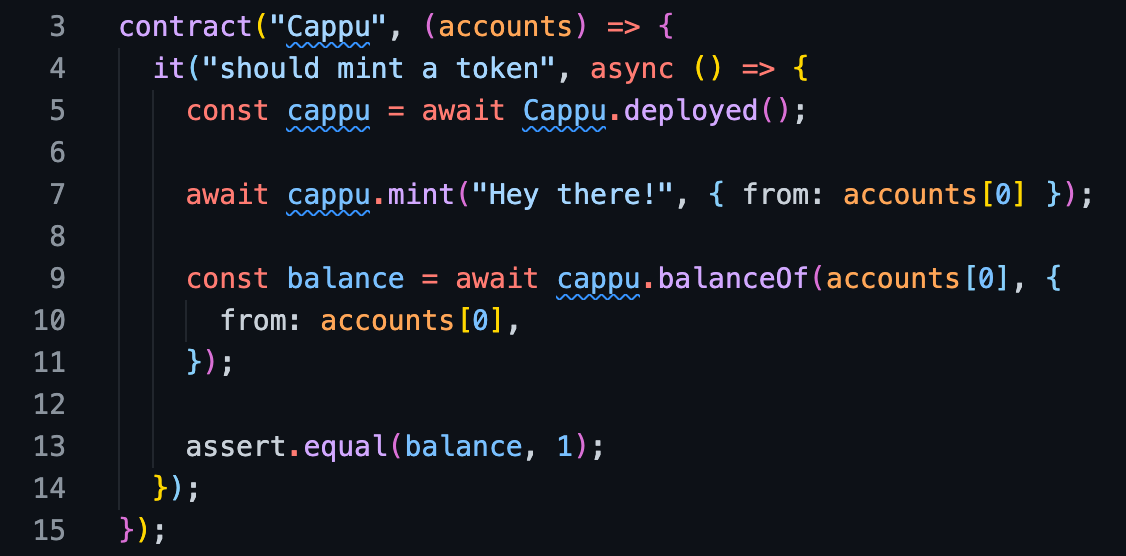
\includegraphics[width=12cm]{mint-test.png}}}
\caption{نمونه یکی از تست‌های قرارداد کاپو}
\label{fig:mint-test}
\end{figure}

پس از نوشته شدن تست‌ها می‌توان آن‌ها را با اجرای دستور
\lr{truffle test}
اجرا کرد.
این دستور پس از اجرای تست‌ها نتیجه و زمان اجرای هر تست را به عنوان خروجی نمایش می‌دهد.
نمونه اجرای این دستور را می‌توان در تصویر
\ref{fig:test-output}
مشاهده کرد.

\begin{figure}
\centerline{\frame{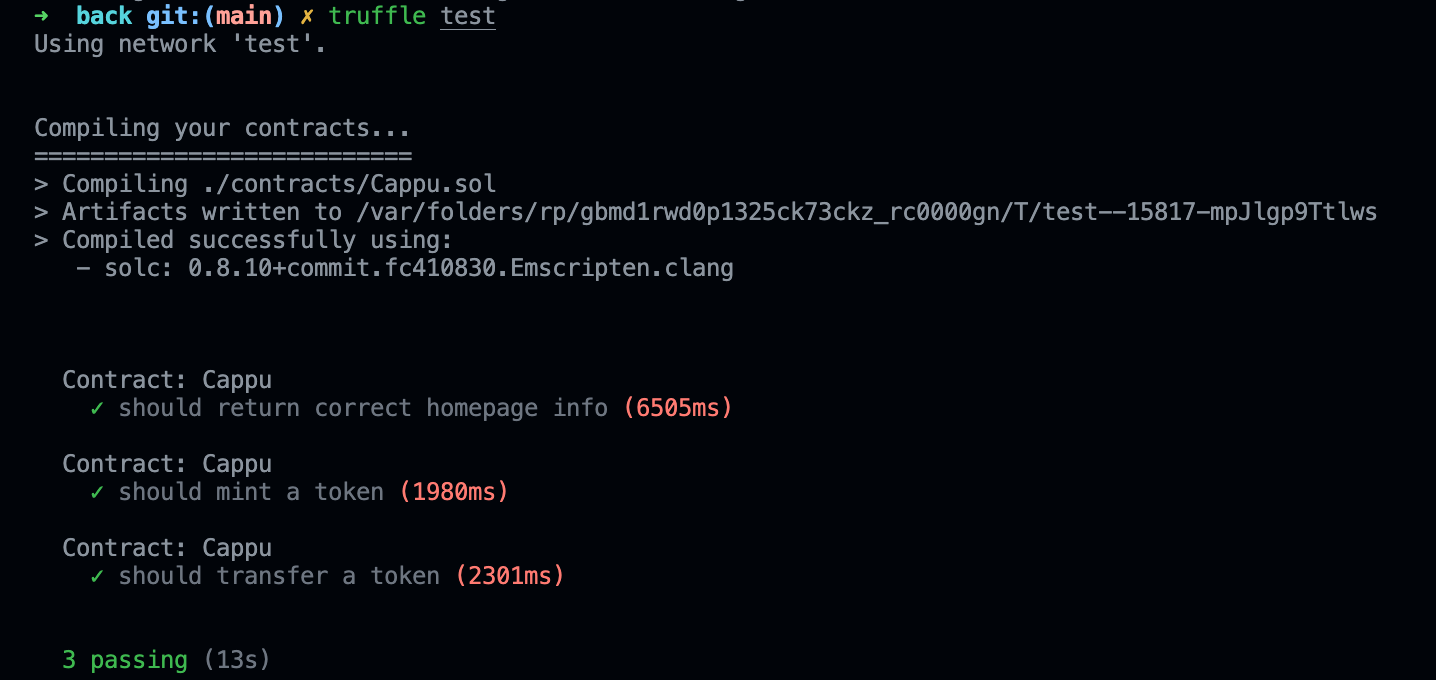
\includegraphics[width=14cm]{test-output.png}}}
\caption{نمونه خروجی اجرای تست‌های قرارداد}
\label{fig:test-output}
\end{figure}

% ------------ Section 4.3
\section{بارگذاری قرارداد روی شبکه تستی \gls{Ropsten}}
تا اینجا قرارداد هوشمند نوشته و تست شده است.
در این مرحله روی شبکه تستی راپستن بارگذاری می‌شود.
فرآیند بارگذاری شدن کاپو به کمک چارچوب ترافل قدم به قدم شرح داده شده است.

\subsection{یافتن آدرس یکی از نُد‌های شبکه برای ارسال تراکنش بارگذاری قرارداد به آن}
آدرس
\gls{Node}
های یک شبکه بلاکچین همه به صورت عمومی در دسترس هستند زیرا نُدها باید بتوانند یکدیگر را ببینند.
راه‌های زیادی برای به دست آوردن آدرس یک نُد وجود دارد.
یکی از آسان‌ترین راه‌های به دست آوردن آدرس یکی از نُد‌های شبکه مراجعه به وبسایت
\gls{Miner}
هاست است.
برای این پروژه مشابه تصویر
\ref{fig:moralis}
از وبسایت مورالیس
\LTRfootnote{
  \url{https://moralis.io}
}
برای پیدا کردن آدرس نُد شبکه استفاده شد.

\begin{figure}
\centerline{\frame{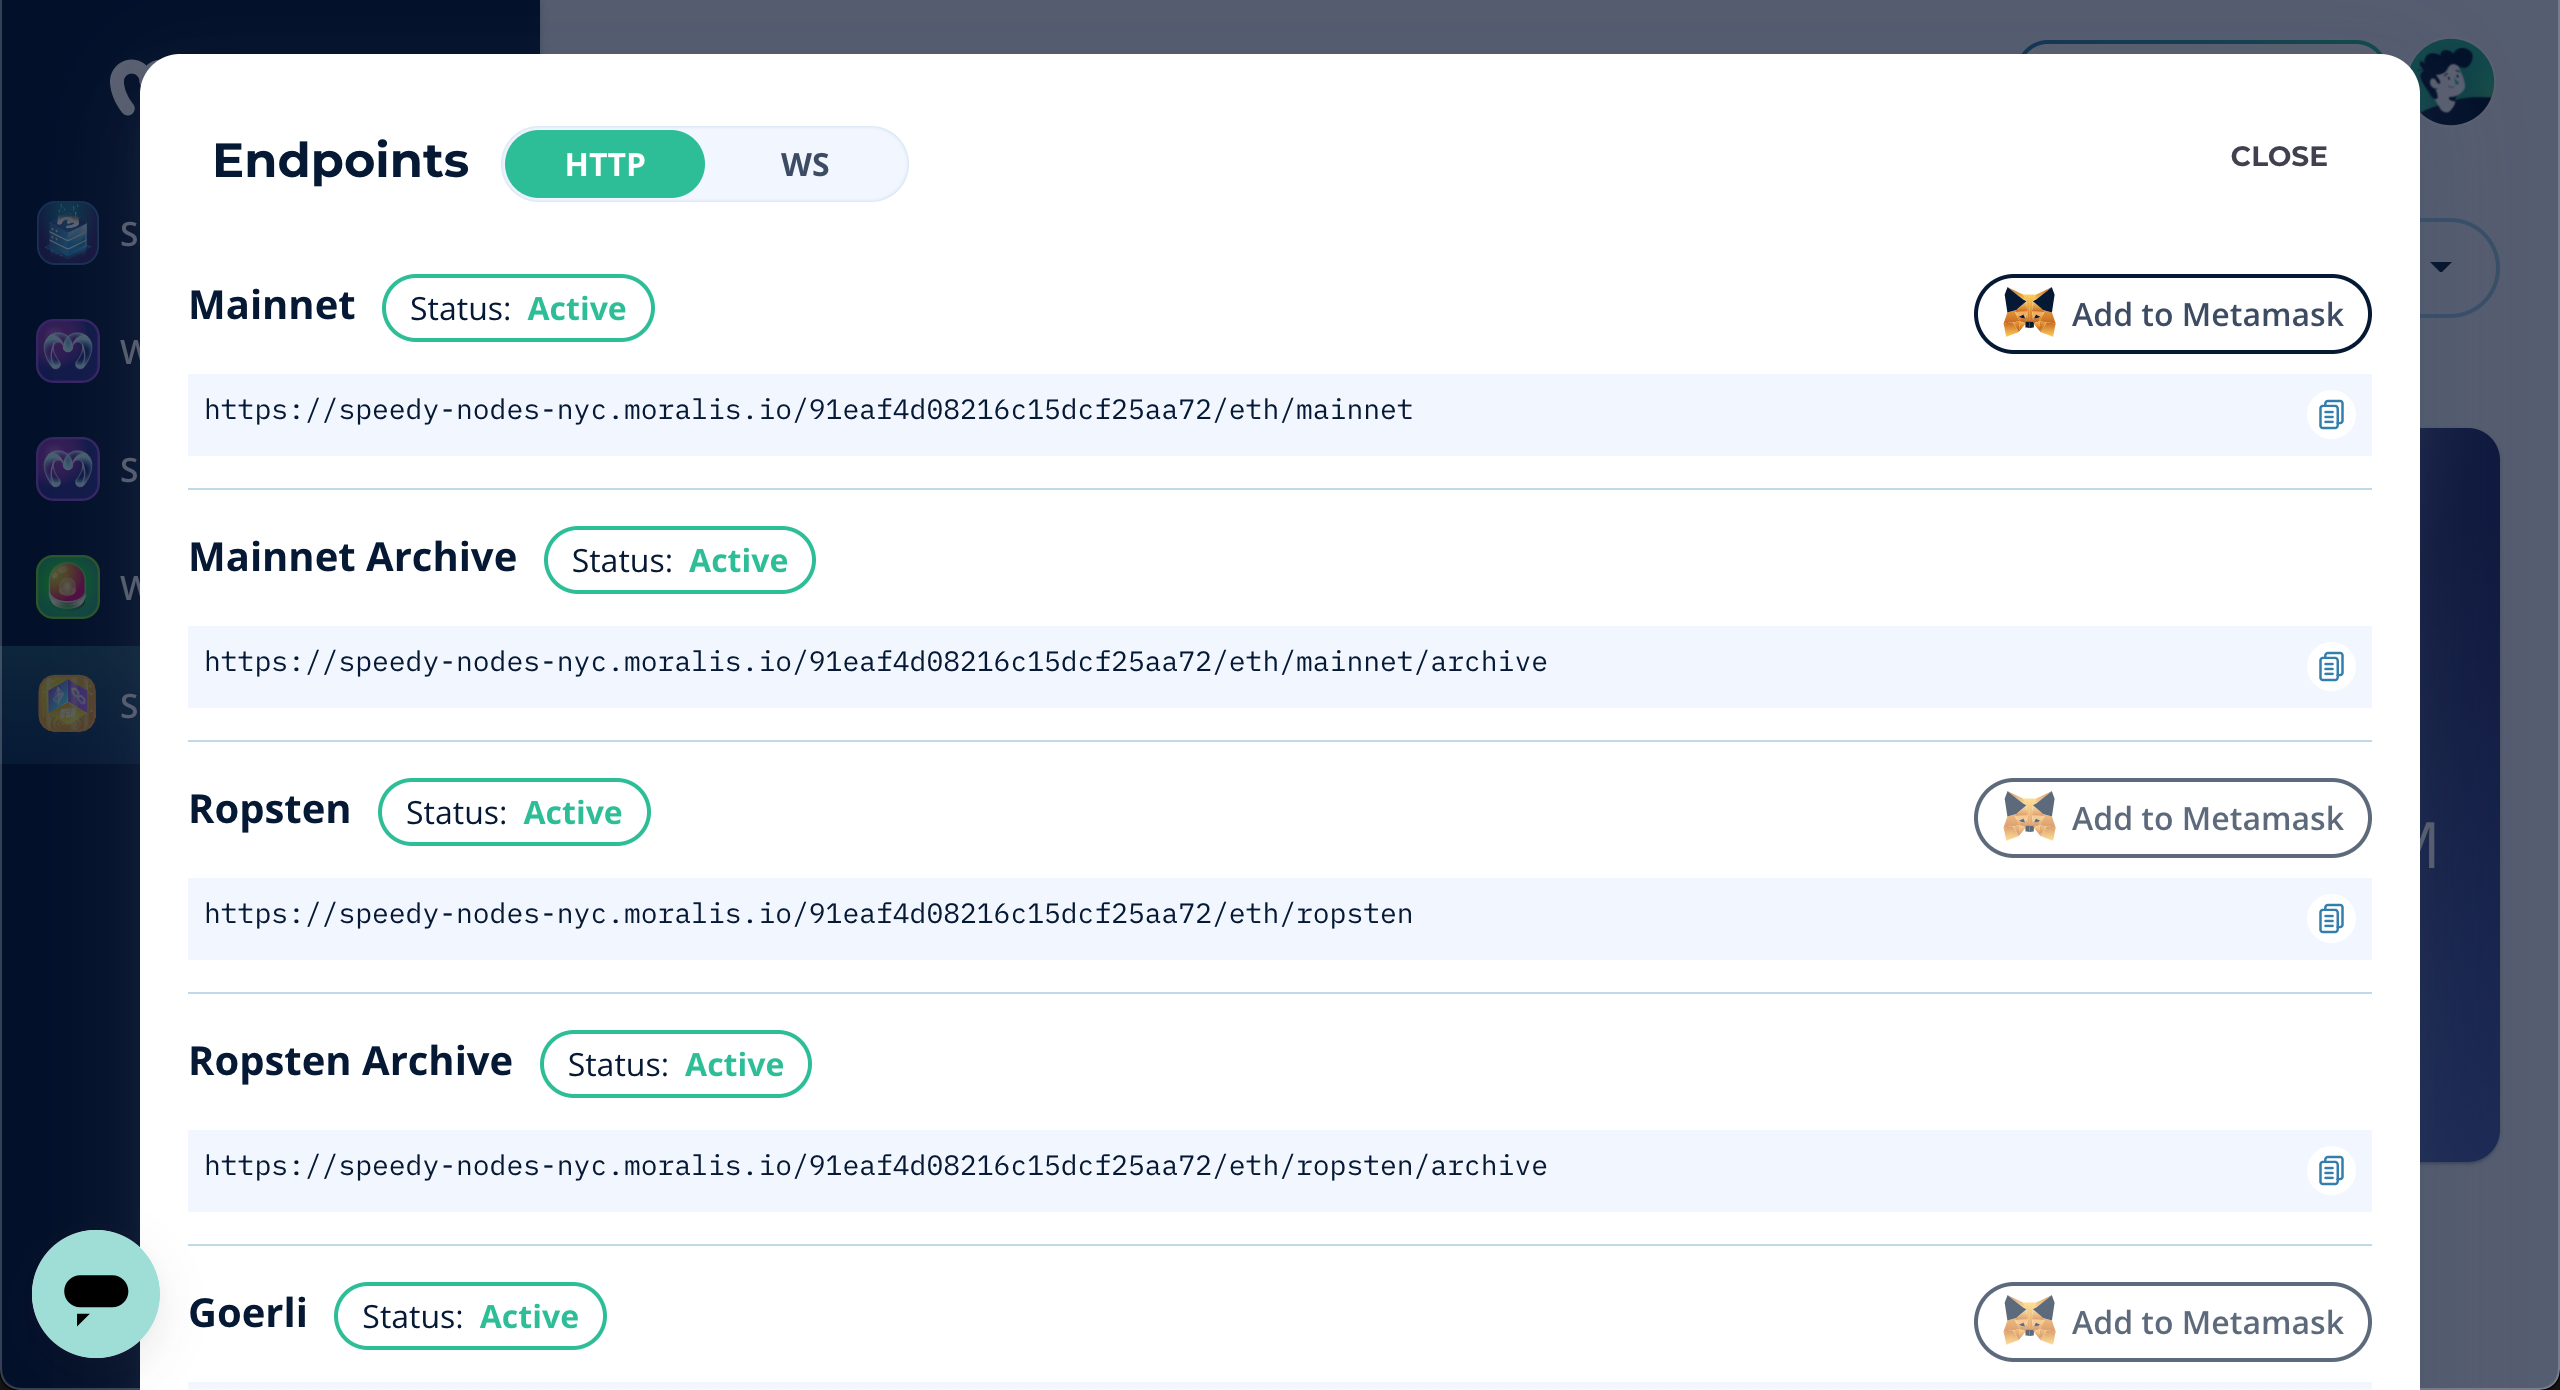
\includegraphics[width=14cm]{moralis.png}}}
\caption{دریافت آدرس یکی از نُد‌های شبکه از وبسایت مورالیس}
\label{fig:moralis}
\end{figure}

\subsection{اضافه شدن اطلاعات شبکه مورد نظر به تنظیمات ترافل}
هنگامی که به کمک دستور
\lr{truffle init}
یک پروژه ترافل ساخته می‌شود، فایلی با نام
\lr{truffle-config.js}
نیز در پوشه‌ی اصلی پروژه ساخته می‌شود.
تنظیمات مربوط به ترافل در این فایل قرار دارند.
برای این که ترافل شبکه مورد نظر را بشناسد باید اطلاعات آن شبکه در این فایل نوشته و شبکه‌ی جدیدی تعریف شود.
برای تعریف شبکه از آدرسی که در گام قبل به دست آمد استفاده می‌شود و مانند تصویر
\ref{fig:network-config}
شبکه‌ی جدیدی تعریف می‌شود.

\begin{figure}
\centerline{\frame{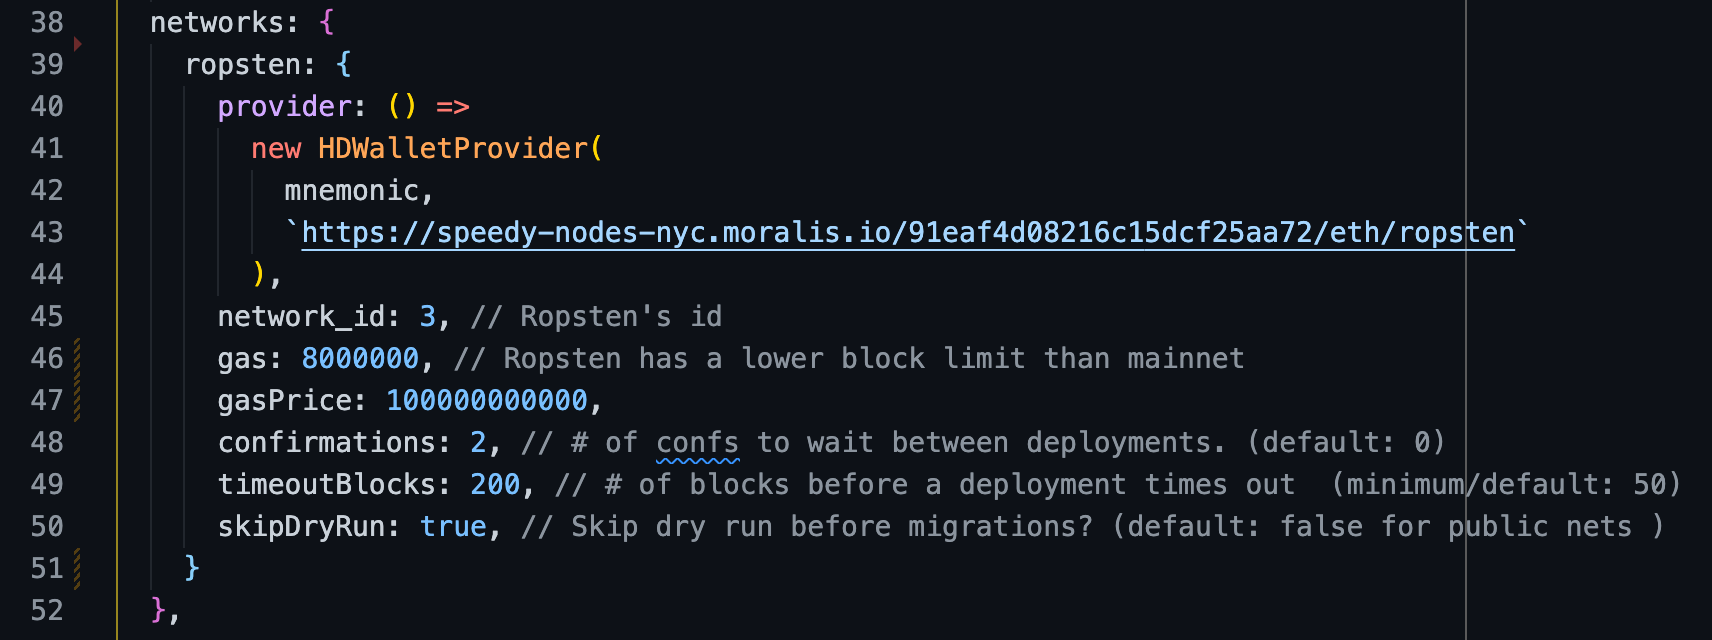
\includegraphics[width=14cm]{network-config.png}}}
\caption{اضافه کردن شبکه راپستن به شبکه‌های ترافل}
\label{fig:network-config}
\end{figure}


\subsection{آماده شدن \gls{Mnemonics}}
برای انجام این پروژه به کمک دستور
\lr{npm mnemonics}
مطابق تصویر
\ref{fig:mnemonics}
یک آدرس تستی ساخته می‌شود.
این دستور، نمونیکز متناسب با این آدرس را به عنوان خروجی می‌دهد. دقت کنید که برای بارگذاری روی
\gls{Mainnet}
حتما باید از نمونیکز مربوط به یک کیف پول واقعی استفاده شود و اطلاعات ان در اختیار کسی قرار نگیرد.

\begin{figure}
\centerline{\frame{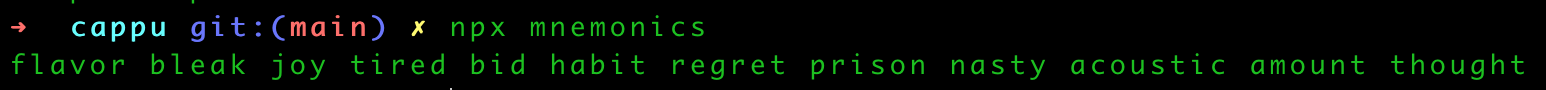
\includegraphics[width=14cm]{mnemonics.png}}}
\caption{ایجاد نمونیکز تستی}
\label{fig:mnemonics}
\end{figure}


\subsection{استفاده از کیف پول ایجاد شده در تنظیمات ترافل}
ترافل برای این که بتواند از کیف‌پول برای انجام تراکنش‌ها استفاده کند باید به نمونیکز یا کلید خصوصی آن دسترسی داشته باشد.
به این منظور فایلی با نام
\lr{secrets.json}
در دایرکتوری اصلی برنامه ساخته می‌شود و مطابق تصویر
\ref{fig:mnemonics-in-secrets}
نمونیکز کیف پول به شکل زیر در آن قرار داده می‌شود.

\begin{figure}
\centerline{\frame{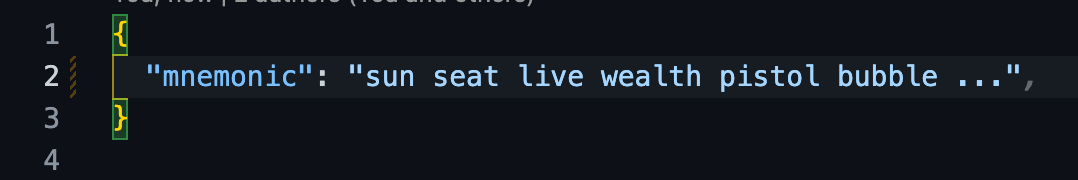
\includegraphics[width=12cm]{mnemonics-in-secrets.png}}}
\caption{قراردادن نمونیکز در فایل secrets.json}
\label{fig:mnemonics-in-secrets}
\end{figure}

سپس در تنظیمات ترافل باید مطابق تصویر
\ref{fig:secrets-in-config}
ذکر شود که می‌تواند آدرس کیف‌پول را در این آدرس پیدا کند.

\begin{figure}
\centerline{\frame{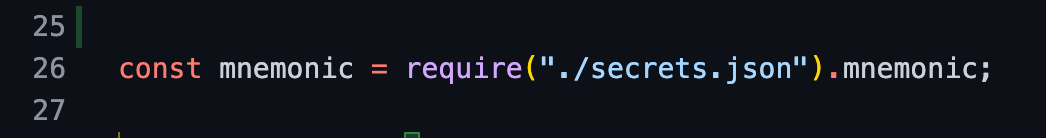
\includegraphics[width=12cm]{secrets-in-config.png}}}
\caption{معرفی فایل secrets.json در تنظیمات ترافل}
\label{fig:secrets-in-config}
\end{figure}


\subsection{نصب کیف‌پول hdwallet}
ترافل برای استفاده از نمونیکز کیف پول ما نیاز به نصب بسته
\lr{hdwallet-provider}
دارد،
این بسته کاربری‌های یک کیف پول دیجیتال از جمله امضا و ارسال تراکنش بر روی شبکه بلاکچین را در اختیار ترافل قرار می‌دهد.
این بسته با اجرای دستور
\lr{npm install –save-dev @truffle/hdwallet-provider}
نصب می‌شود.  پس از نصب کیف پول در تنظیمات ترافل در فایل
\lr{truffle-config.js}
مطابق با تصویر
\ref{fig:wallet-in-config}
ذکر می‌شود که از این کیف‌پول استفاده شود.

\begin{figure}
\centerline{\frame{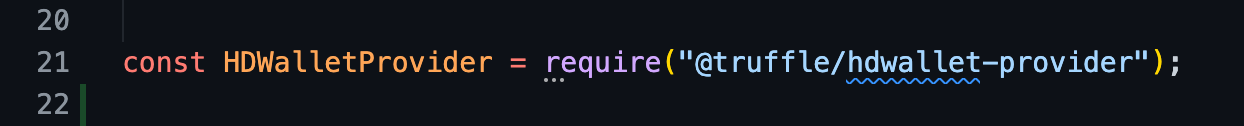
\includegraphics[width=12cm]{wallet-in-config.png}}}
\caption{استفاده از کیف‌پول hdwallet در تنظیمات ترافل}
\label{fig:wallet-in-config}
\end{figure}


\subsection{انتخاب شبکه اضافه شده}
حال هنگام ورود به خط فرمان ترافل مانند تصویر
\ref{fig:truffle-console}
شبکه مورد نظر انتخاب می‌شود.

\begin{figure}
\centerline{\frame{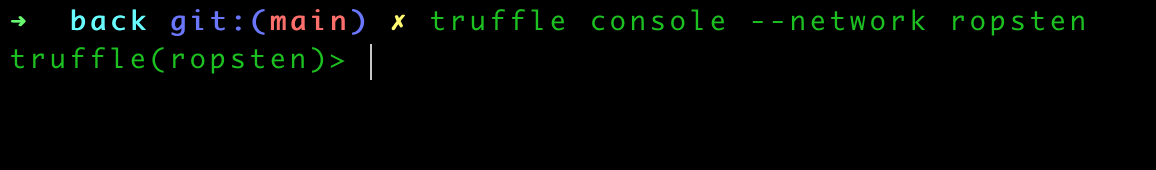
\includegraphics[width=12cm]{truffle-console.png}}}
\caption{ورود به خط فرمان ترافل با انتخاب شبکه راپستن}
\label{fig:truffle-console}
\end{figure}


\subsection{بررسی آدرس کیف‌پول و موجودی آن}
برای بارگذاری یک قرارداد هوشمند باید آدرس بارگذاری کننده آن بتواند هزینه تراکنش بارگذاری را پرداخت کند.
در صورتی که بارگذاری بر روی یک شبکه تستی انجام می‌شود باید با استفاده از یک
\lr{faucet}
روی شبکه تستی به میزان کافی پول تستی دریافت شود.

برای دریافت آدرس‌های کیف‌پول مانند تصویر
\ref{fig:get-addresses}
از دستور
\lr{getAccounts}
در خط فرمان ترافل استفاده می شود.
همچنین برای دریافت مانده حساب آدرس، مانند تصویر
\ref{fig:get-wallet-balance}
از دستور
\lr{getBalance}
در خط فرمان ترافل استفاده می‌شود.

\begin{figure}
\centerline{\frame{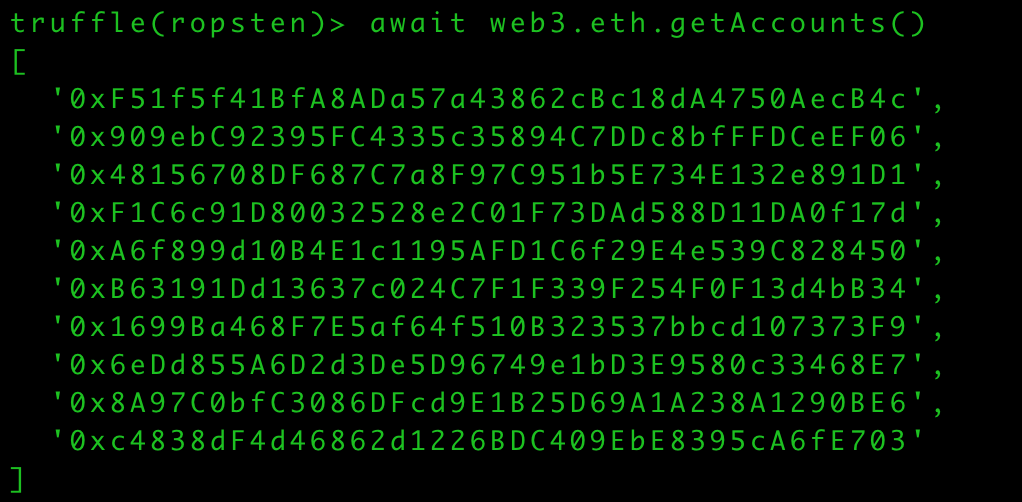
\includegraphics[width=12cm]{get-addresses.png}}}
\caption{دریافت آدرس‌های کیف‌پول در خط فرمان ترافل}
\label{fig:get-addresses}
\end{figure}

\begin{figure}
\centerline{\frame{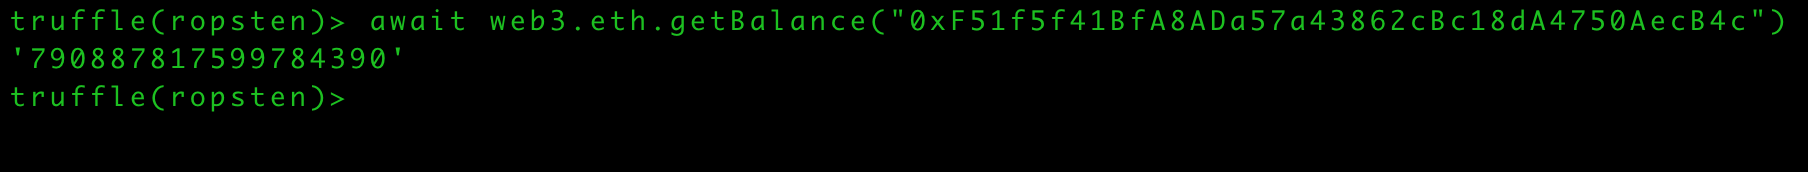
\includegraphics[width=14cm]{get-wallet-balance.png}}}
\caption{دریافت موجودی کیف‌پول در خط فرمان ترافل}
\label{fig:get-wallet-balance}
\end{figure}


\subsection{بارگذاری قرارداد هوشمند روی شبکه بلاکچین}
پس از اطمینان از توانایی پرداخت کارمزد تراکنش با استفاده از دستور
\lr{migrate}
در خط فرمان ترافل قرارداد هوشمند روی شبکه بلاکچین بارگذاری می‌شود.


\subsection{اطمینان از صحت بارگذاری قرارداد هوشمند}
پس از اتمام بارگذاری قرارداد هوشمند برای اطمینان از به درستی انجام شدن فرآیند بارگذاری قرارداد،
می‌توان از
\glspl{Block Explorer}
بلاکچین استفاده کرد.
برای مثال قرارداد هوشمند کاپو بر روی شبکه راپستن بارگذاری شده است، که با رفتن به وبسایت اتراسکن
\LTRfootnote{
\url{https://etherscan.io}
}
و قراردادن آن روی شبکه راپستن، مانند تصویر
\ref{fig:etherscan}
می‌توان قرارداد بارگذاری شده و تراکنش‌های آن را مشاهده کرد.


\begin{figure}
\centerline{\frame{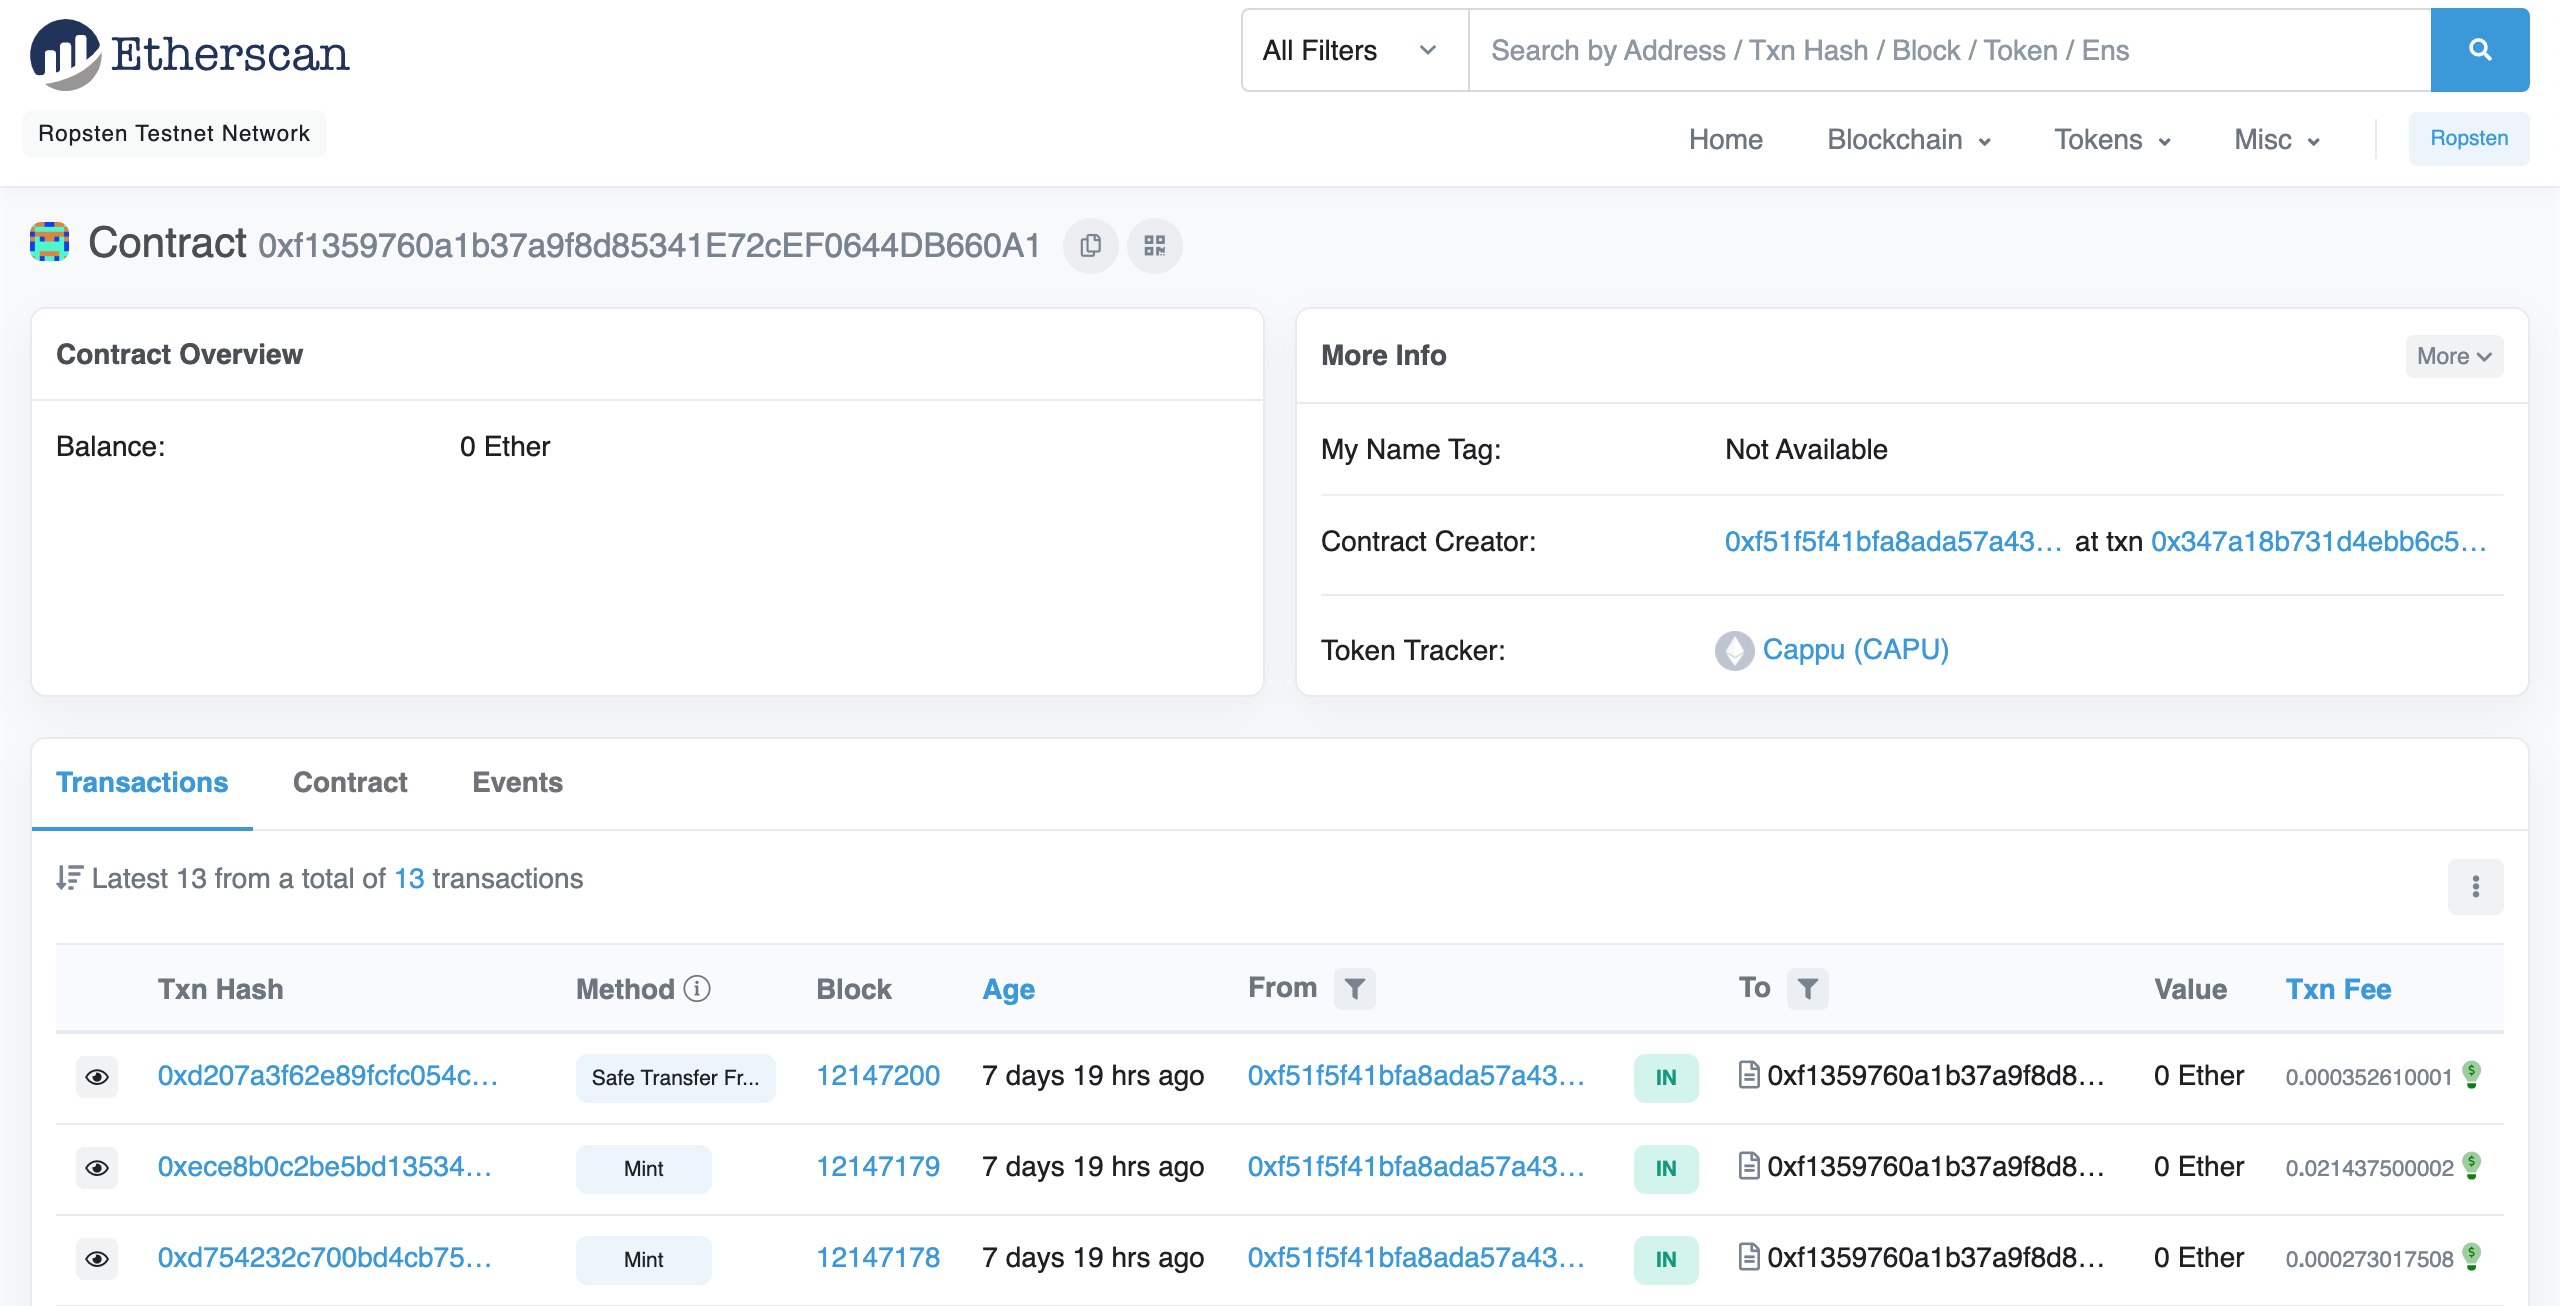
\includegraphics[width=14cm]{etherscan.png}}}
\caption{مشاهده قراداد کاپو در اتراسکن روی شبکه راپستن}
\label{fig:etherscan}
\end{figure}


% ------------ Section 4.4
\section{توسعه واسط‌کاربری}
برای توسعه واسط‌کاربری اپلیکیشن،
\gls{React}
به عنوان چارچوب مورد استفاده انتخاب شده است.
ترکیب این چارچوب با استفاده از کتابخانه
\lr{material-ui}
که کمک می‌کند در زمان کوتاه بتوان ظاهری زیبا و یکدست در اپلیکیشن ایجاد کرد و کتابخانه
\lr{Web3JS}
که واسط‌کاربری را به کیف پول کاربر و شبکه بلاکچین متصل می‌کند،
همه‌ی قابلیت‌های مورد نیاز برای توسعه یک واسط‌کاربری زیبا و کارآمد را در اختیار توسعه‌دهنده قرار می‌دهد.

\subsection{اتصال به کیف پول و قرارداد کاپو}
در پوشه اصلی واسط‌کاربری فایلی با عنوان
\lr{config.js}
وجود دارد.
در این فایل علاوه بر
\lr{ABI}\LTRfootnote{Application Binary Interface}
قرارداد هوشمند سایر اطلاعات مورد نیاز مانند آدرس شبکه،
آدرس قرارداد در شبکه و نام شبکه مورد نظر نیز ذخیره می‌شود.
هنگام توسعه باید دقت شود که این فایل به قرارداد روی شبکه محلی اشاره کند.

برای استفاده از کتابخانه‌ی
\lr{Web3JS}
و اتصال به کیف‌پول کاربر یک فایل به نام
\lr{connect.js}
ساخته شد.
تمامی اعمال ارتباطی با کیف پول کاربر به عنوان چند تابع در این فایل جمع آوری شده‌اند.
این فایل به صورت یک آداپتور میان
\lr{Web3JS}
و کد کاپو عمل می‌کند. تمامی قابلیت‌های مورد نیاز مانند اتصال به کیف‌پول و
\gls{Login}
کاربر،
\gls{Logout}
کاربر، گرفتن آدرس و شبکه‌ی کیف پول و ... در این فایل انجام می‌شود.

واسط‌کاربری کاپو پس از تایید کاربر و دریافت آدرس کیف‌پول او، آن را در
\lr{sessionStorage}
ذخیره می‌کند،
از این طریق متوجه می شود که آیا کاربر کیف پول خود را به برنامه متصل کرده وارد شده است یا خیر.
کاپو پیش از اتصال به کیف پول کاربر چک می‌کند که کیف پول روی شبکه یکسانی با شبکه فعلی کاپو باشد
و در غیر این صورت مانند تصویر
\ref{fig:cappu-wrong-network-error}
به کاربر هشدار می‌دهد که شبکه‌ی کیف پول را تغییر دهد.

\begin{figure}[H]
\centerline{\frame{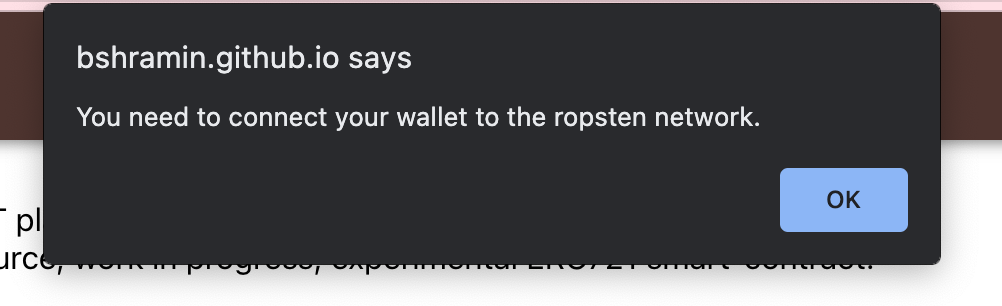
\includegraphics[width=12cm]{cappu-wrong-network-error.png}}}
\caption{پیام کاپو به کاربر هنگامی که کیف پول روی شبکه مورد نظر نباشد.}
\label{fig:cappu-wrong-network-error}
\end{figure}

\subsection{تجربه کاربری}
همچنین در واسط‌کاربری کاپو برای داشتن تجربه کاربری بهتر تلاش شده است.
نکاتی مانند عدم نمایش قابلیت‌هایی مانند ساخت و ارسال توکن هنگامی که کیف پول کاربر به اپلیکیشن متصل نیست،
جابه‌جایی آسان میان صفحات به کمک
\lr{react-router}
، طراحی
\gls{Responsive}
برای رایانه و گوشی موبایل، نمایش
\gls{Alert}
ها و
\gls{Error}
های مناسب به کاربر، نمایش نشانگر
\gls{Loading}
هنگامی که تراکنش‌ها در حالت
\gls{Pending}
هستند و نمایش پیام‌های مناسب با توجه به نتیجه تراکنش‌های کاربر.

در این قسمت روند تعامل یک کاربر با کاپو مورد بررسی قرار می‌گیرد.
هنگامی که کاربر برنامه کاپو را باز می‌کند و هنوز کیف پولش را متصل نکرده است،
مانند تصویر
\ref{fig:homepage-not-loggedin}
توضیحاتی در مورد نحوه عملکرد کاپو
و همچنین آماری از تعداد توکن‌های ساخته شده و تعداد آدرس‌های دارای نوکن را مشاهده می‌کند.
کاربر هنوز گزینه‌هایی مانند ساخت توکن یا لیست توکن‌ها را نمی‌بیند زیرا به آن‌ها دسترسی ندارد.
پس از اتصال کیف‌پول کاربر  به کاپو گزینه‌های ساخت توکن و لیست توکن‌ها مانند تصویر
\ref{fig:homepage-loggedin}
به صفحه اضافه می‌شوند.

\begin{figure}
\centerline{\frame{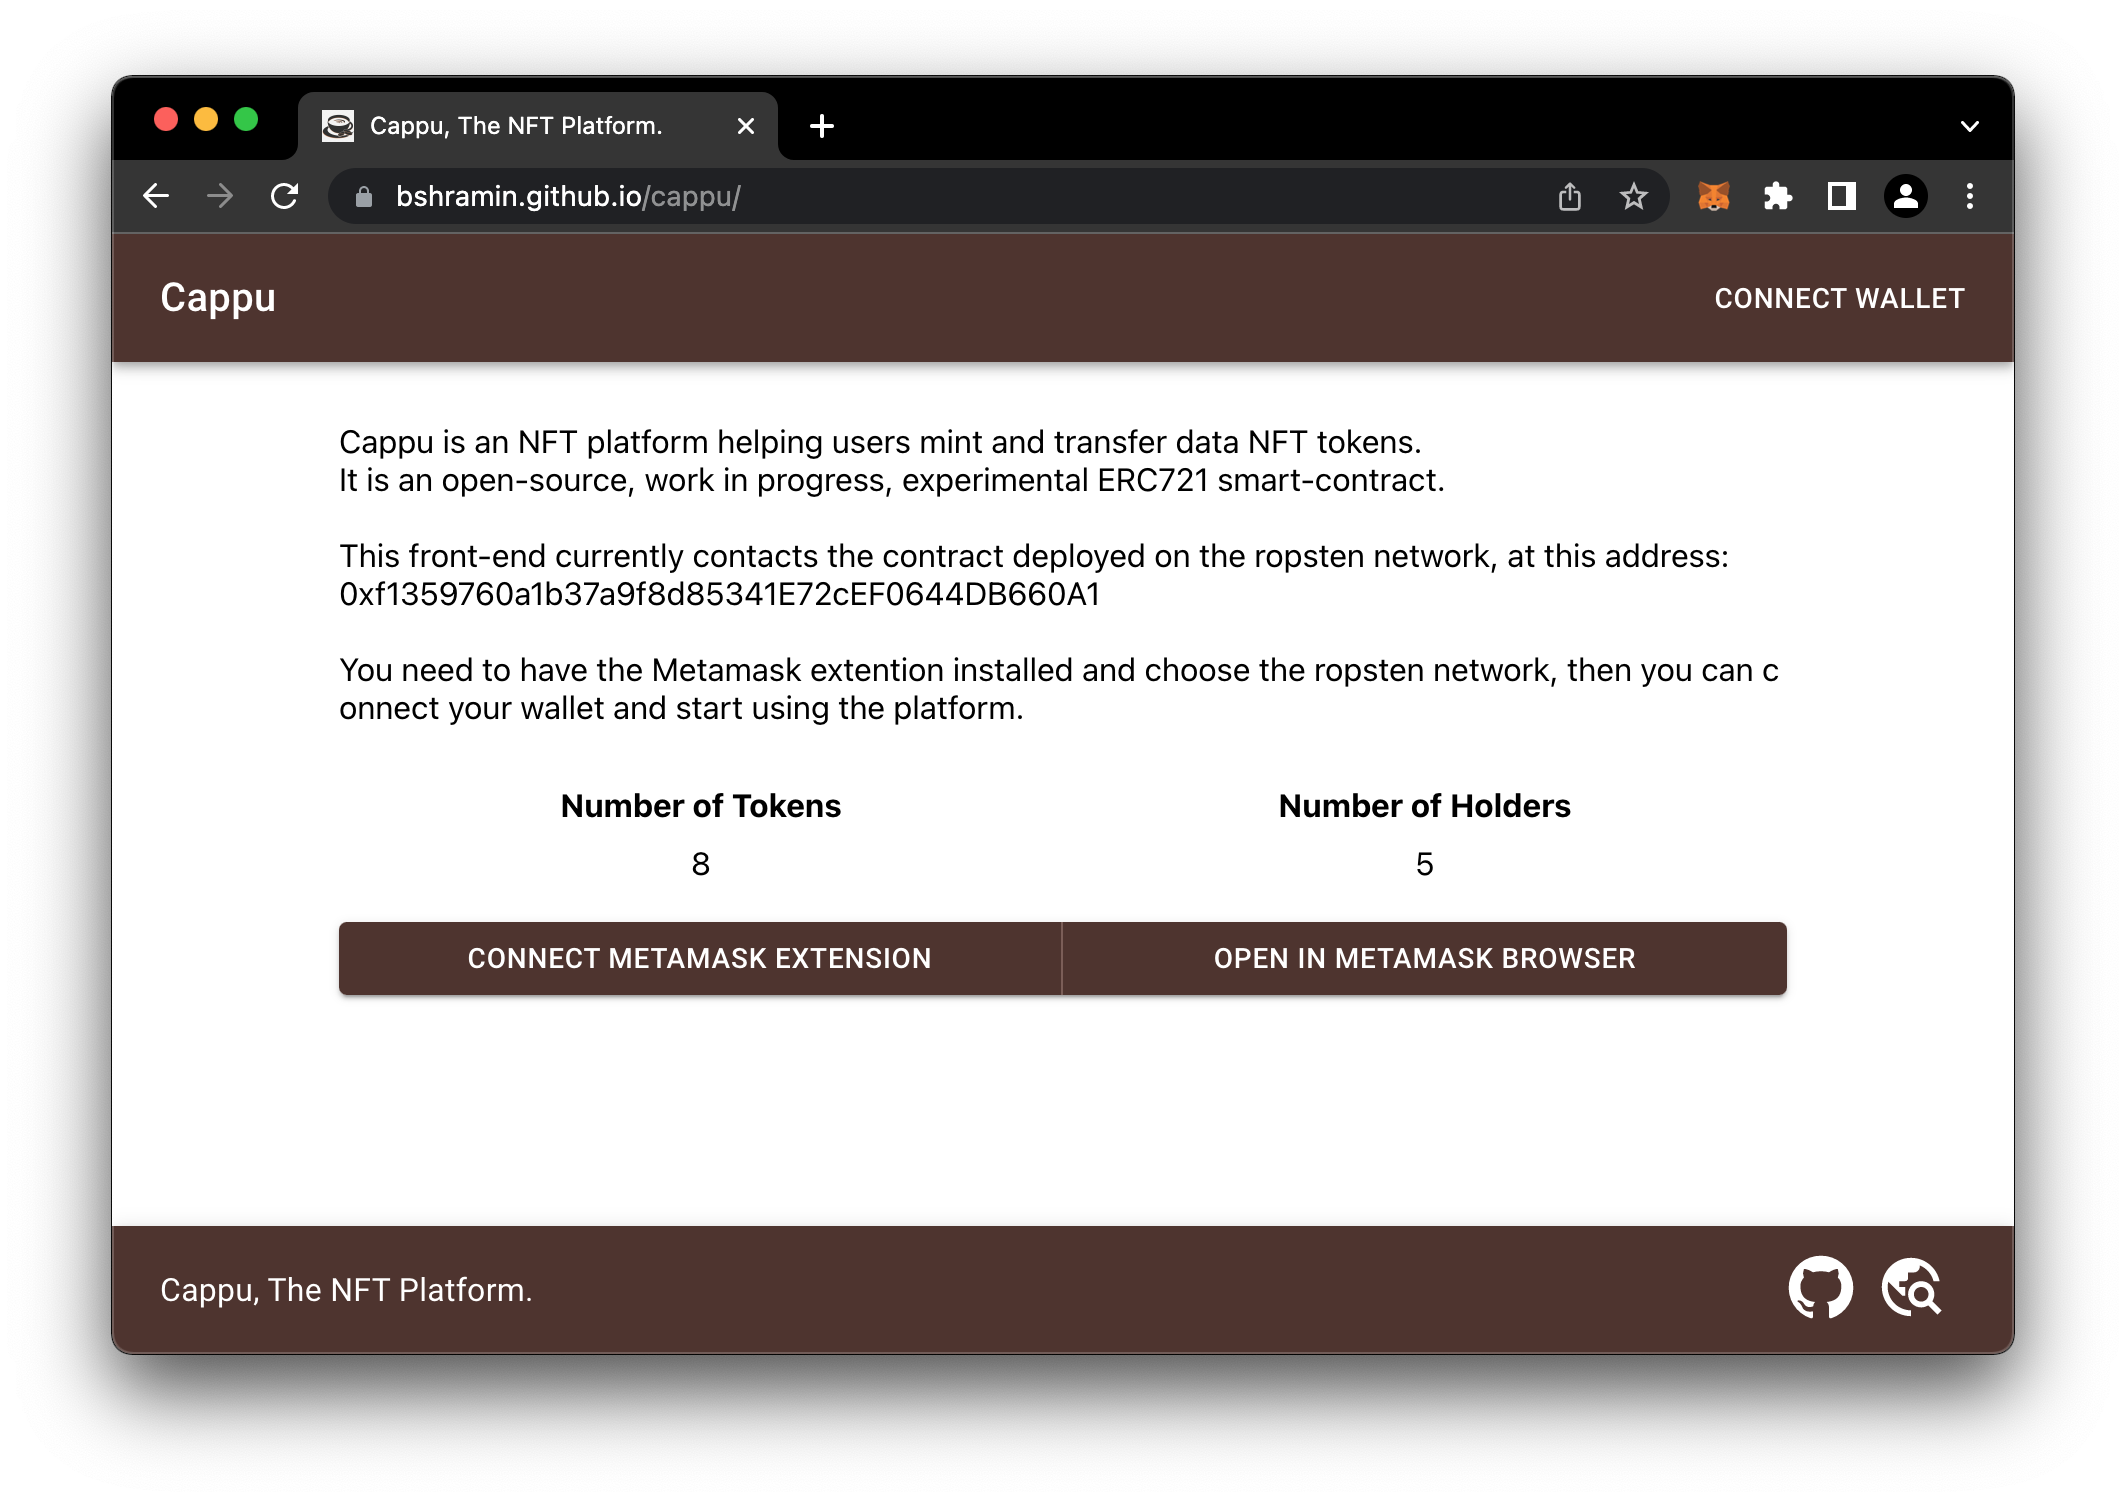
\includegraphics[width=12cm]{homepage-not-loggedin.png}}}
\caption{صفحه اصلی کاپو (بدون کیف پول متصل).}
\label{fig:homepage-not-loggedin}
\end{figure}

\begin{figure}
\centerline{\frame{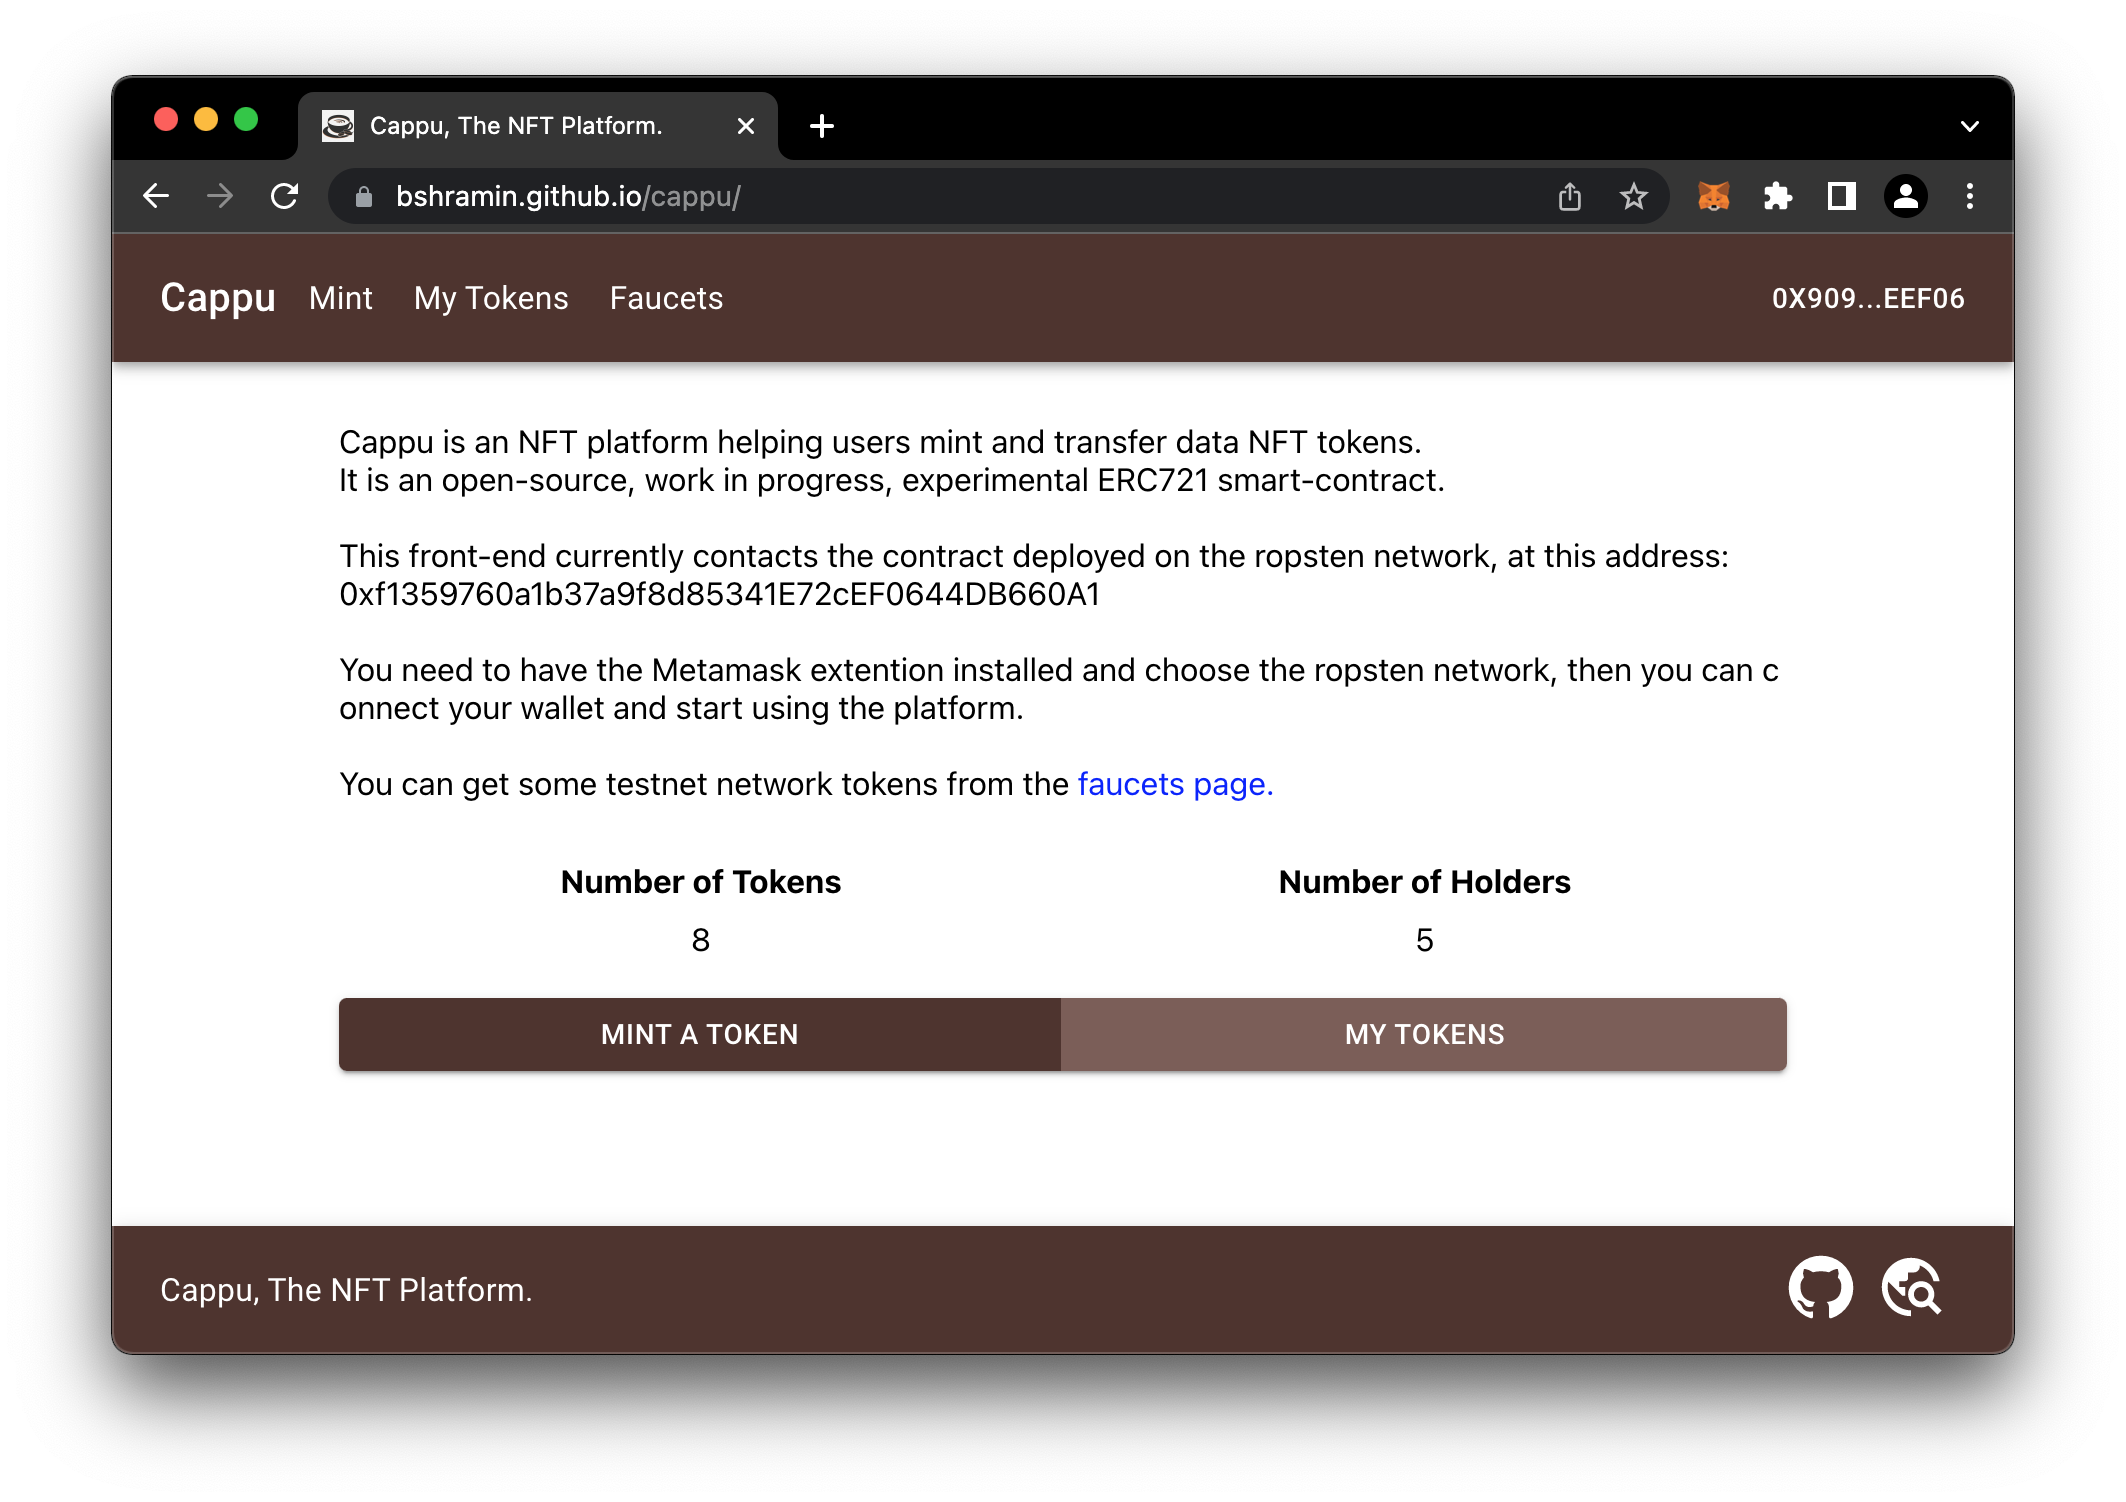
\includegraphics[width=12cm]{homepage-loggedin.png}}}
\caption{صفحه اصلی کاپو (با کیف پول متصل).}
\label{fig:homepage-loggedin}
\end{figure}

حال کاربر که کیف پول خود را به کاپو متصل کرده است می‌تواند توکن بسازد.
برای این منظور از قسمت بالای صفحه گزینه
\lr{Mint}
را انتاخب می‌کند.
در صفحه‌ای که باز می‌شود اطلاعات توکن را وارد کرده و دکمه
\lr{Mint}
را می‌زند.
حال کاپو تراکنش ساخت توکن را به کیف پول کاربر می‌فرستد که توسط کاربر تایید و روی شبکه ارسال شود.
تا زمانی که نتیجه‌ی تراکنش مشخص نشده است کاپو مانند تصویر
\ref{fig:mint-loading}
پیام انتظار به کاربر نمایش می‌دهد.
سپس در صورت موفقیت آمیز بودن ساخت توکن، مانند تصویر
\ref{fig:mint-success}
پیام مناسب به کاربر نمایش داده می‌شود.

\begin{figure}
\centerline{\frame{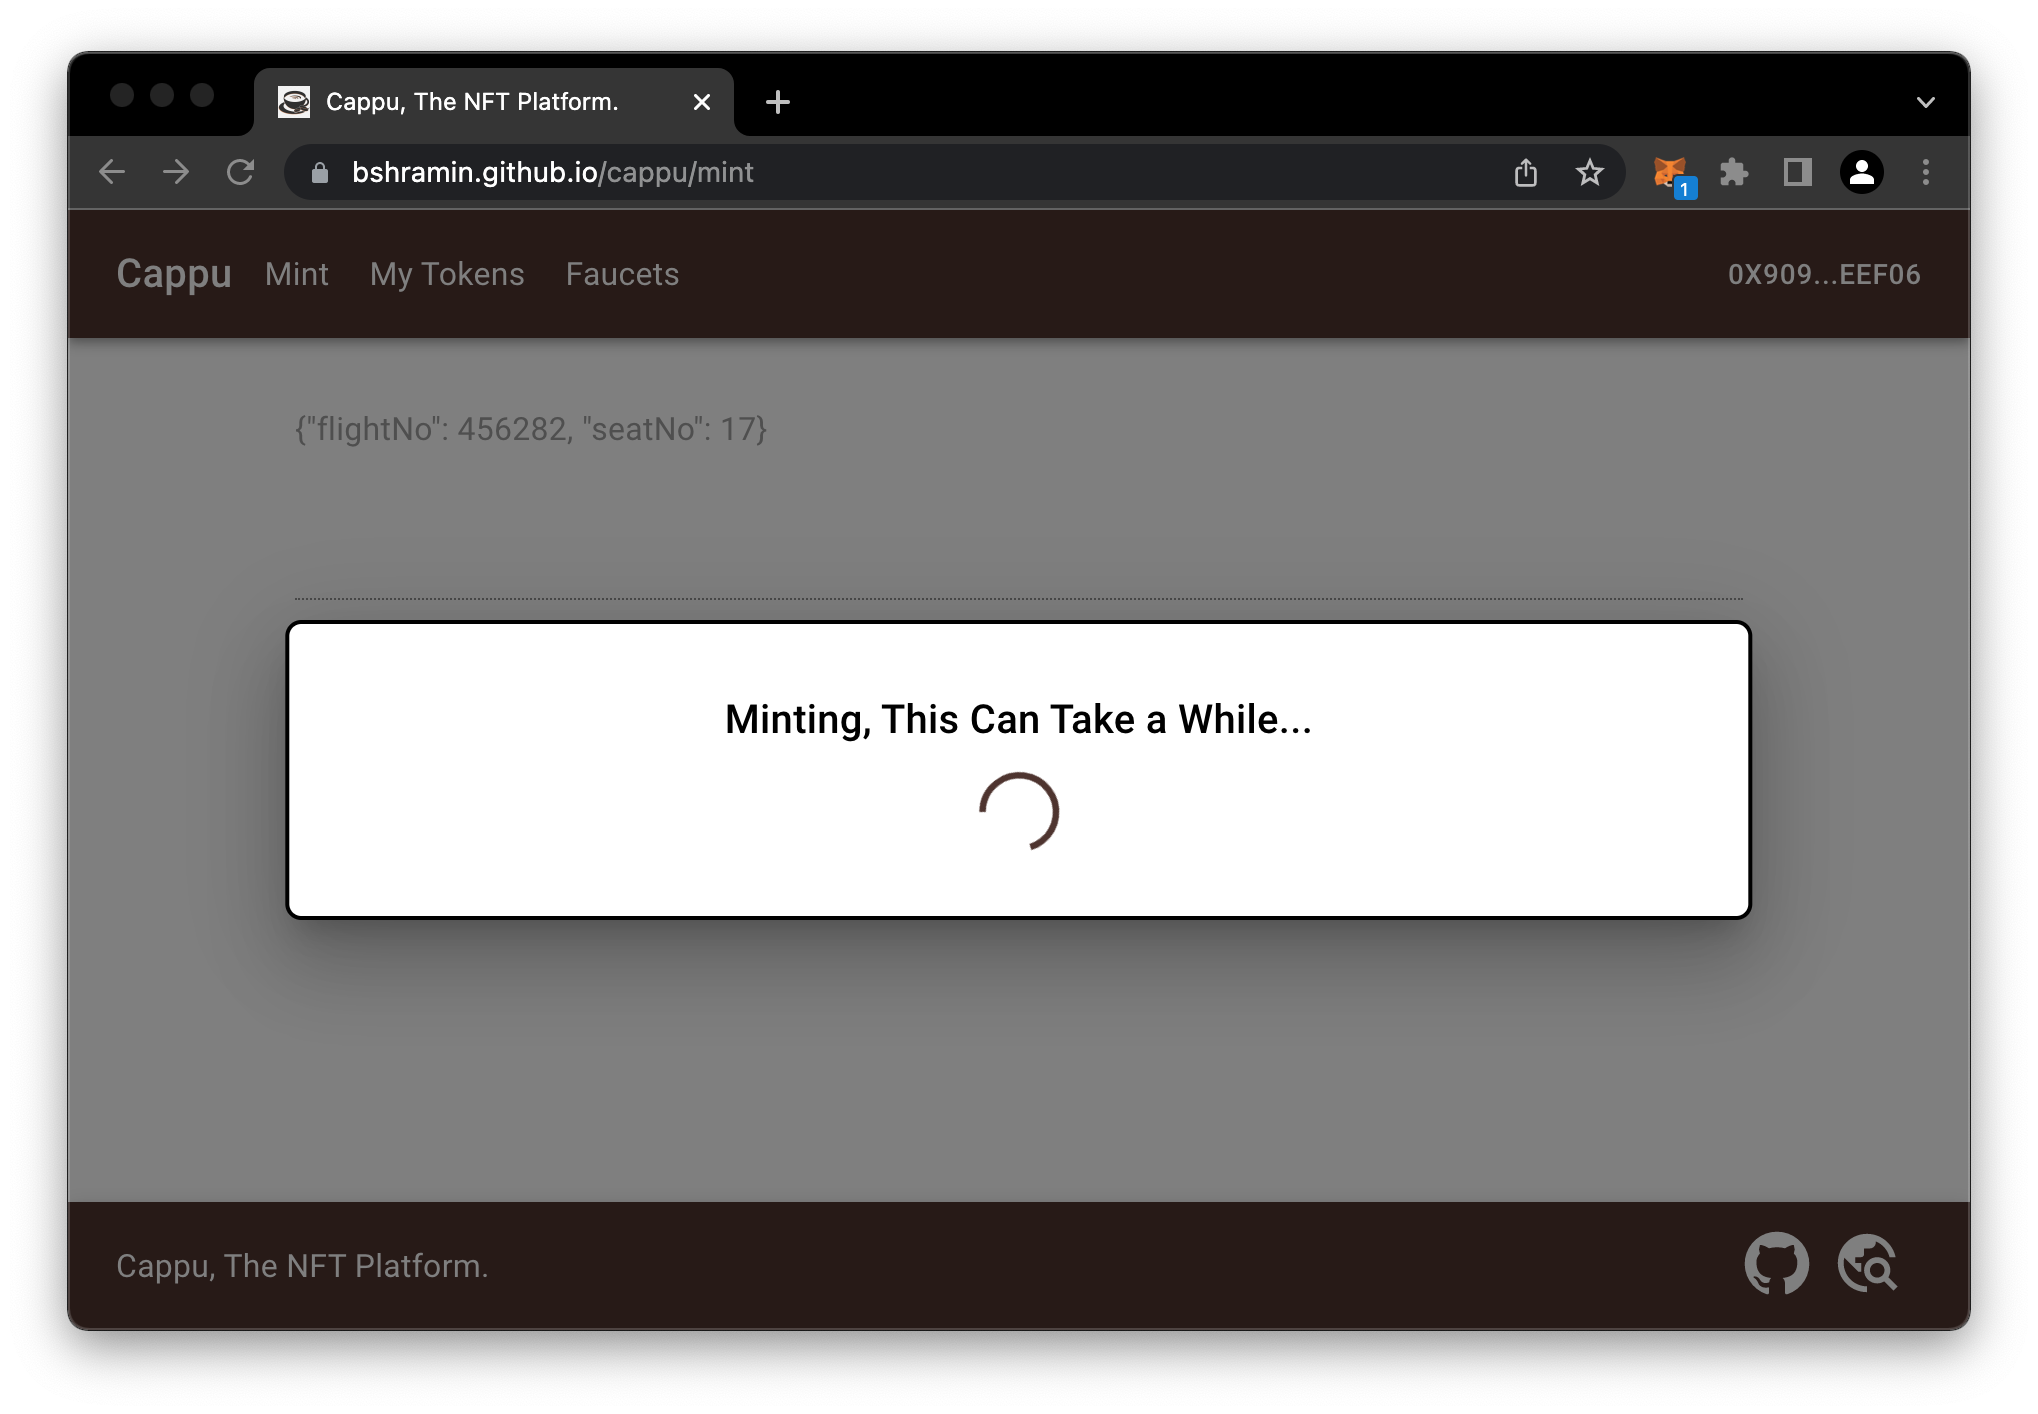
\includegraphics[width=12cm]{mint-loading.png}}}
\caption{کاپو در حال ساخت توکن.}
\label{fig:mint-loading}
\end{figure}

\begin{figure}
\centerline{\frame{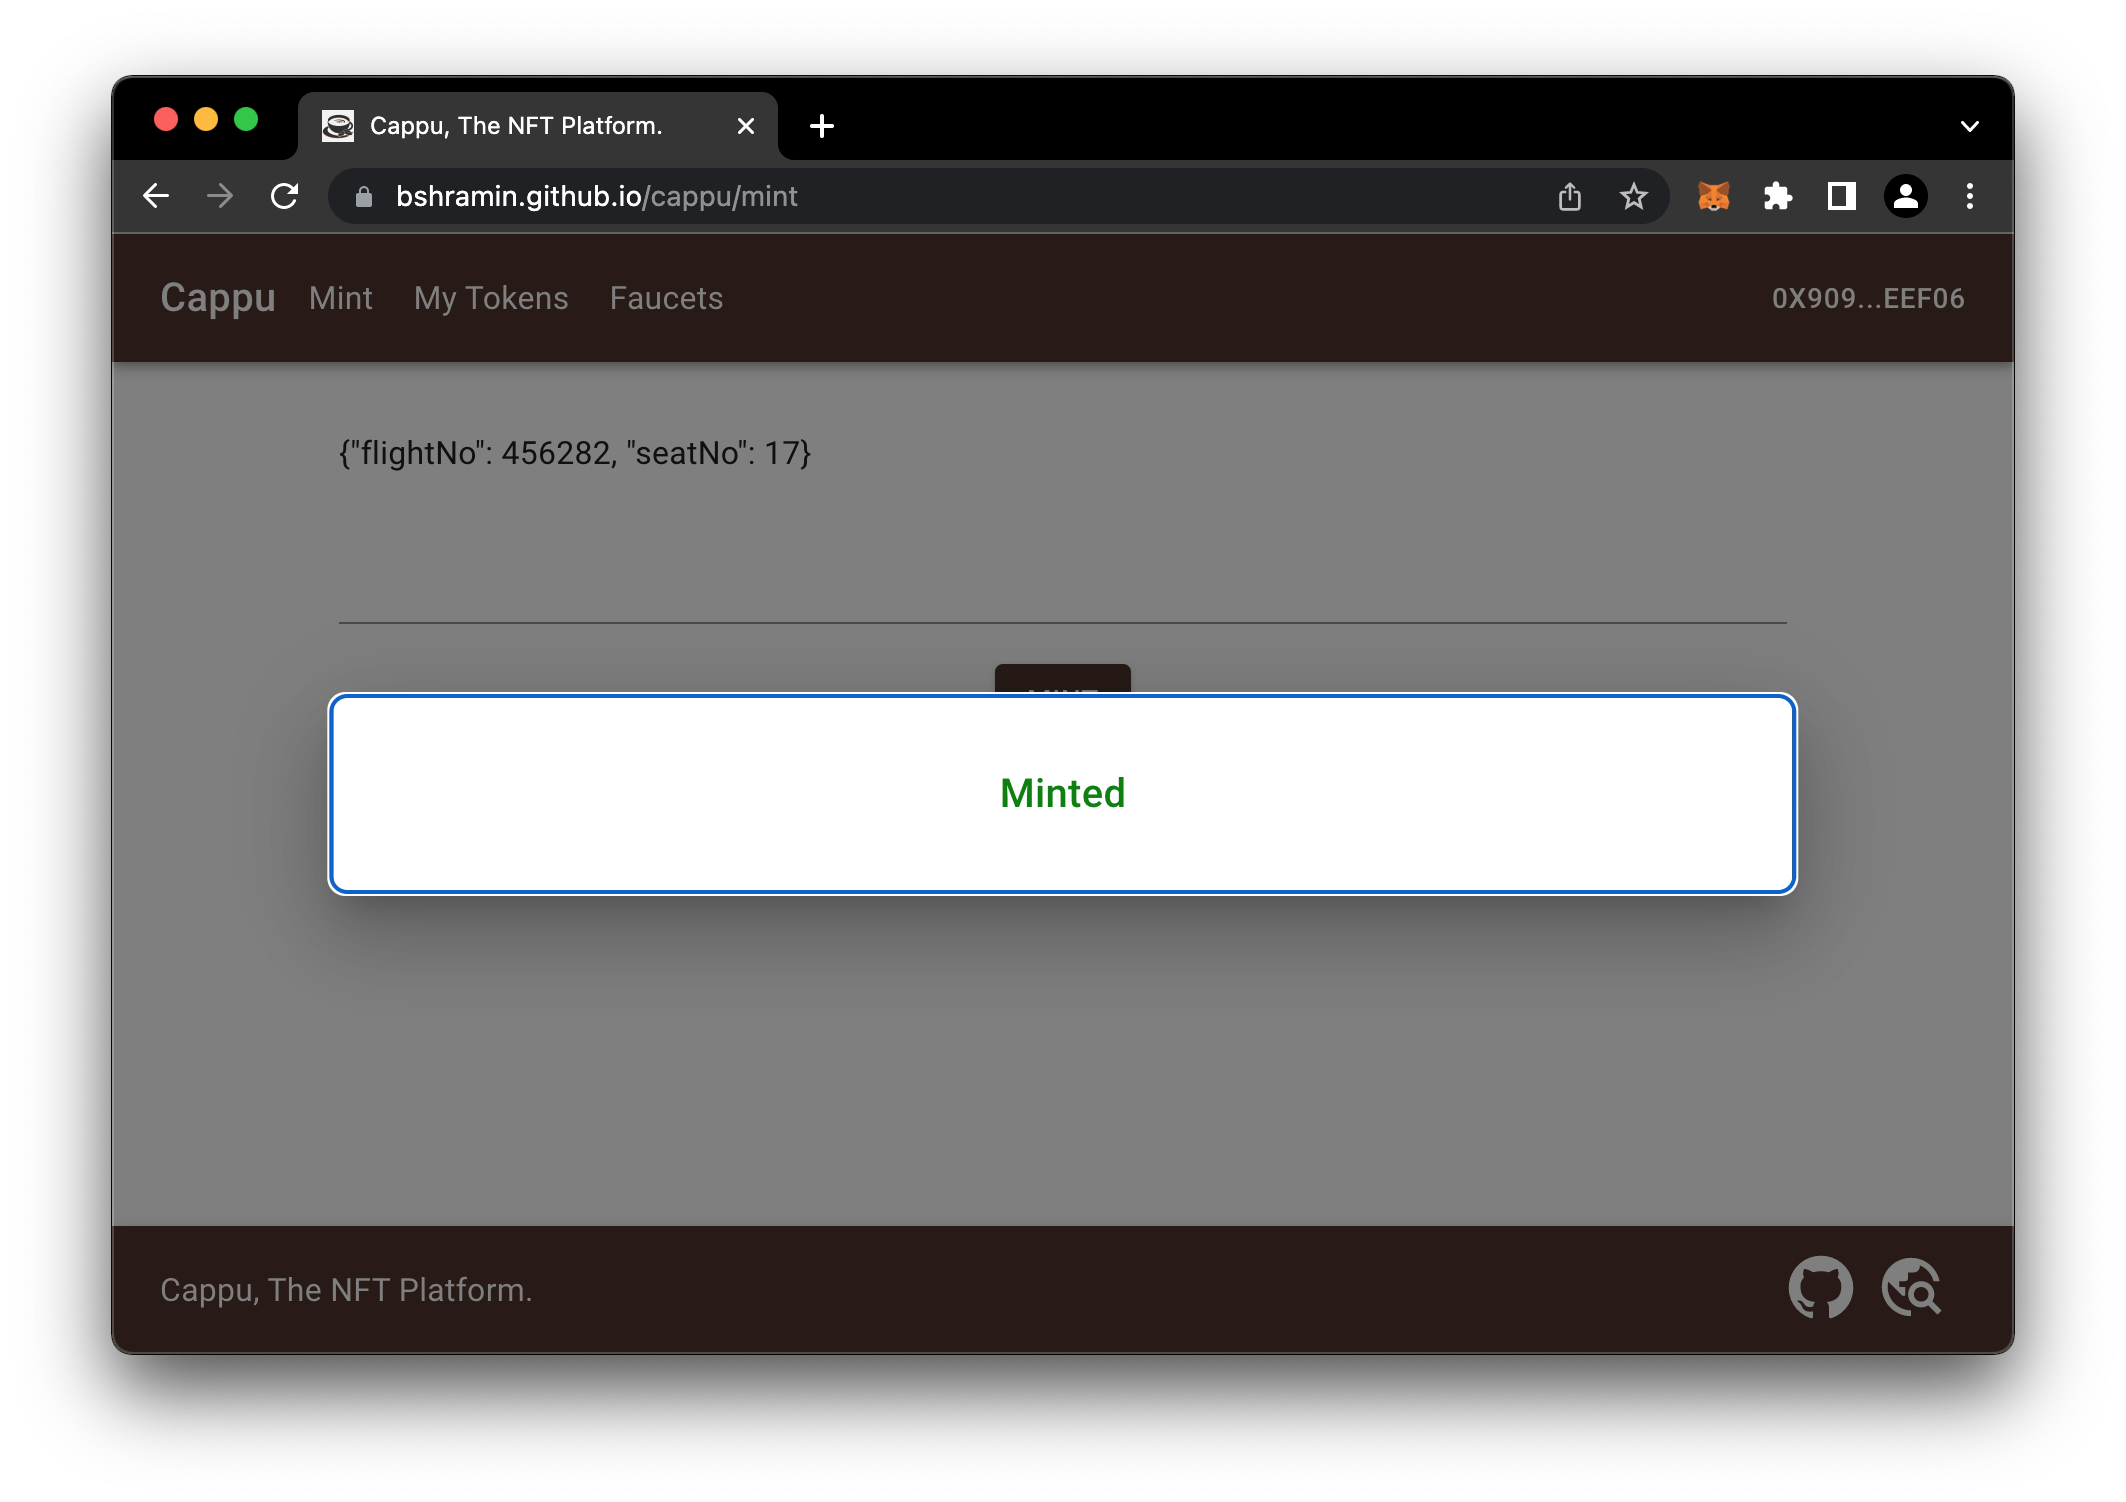
\includegraphics[width=12cm]{mint-success.png}}}
\caption{پیام موفقیت در ساخت توکن.}
\label{fig:mint-success}
\end{figure}

پس از ساخت یک یا چند توکن، کاربر می‌تواند با انتخاب گزینه
\lr{My Tokens}
یه صفحه لیست توکن‌ها منتقل شود.
در این قسمت کاربر می‌تواند دارایی‌هایش را مشاهده کند.
در صورتی که کاربر دارای توکنی نباشد پیام مناسب مانند تصویر
\ref{fig:no-tokens-yet}
به کاربر نمایش داده می‌شود.
در صورتی که کاربر توکن‌هایی داشته باشد نیز مانند تصویر
\ref{fig:tokens-list}
لیست توکن‌هایش را مشاهده می‌کند.


\begin{figure}
\centerline{\frame{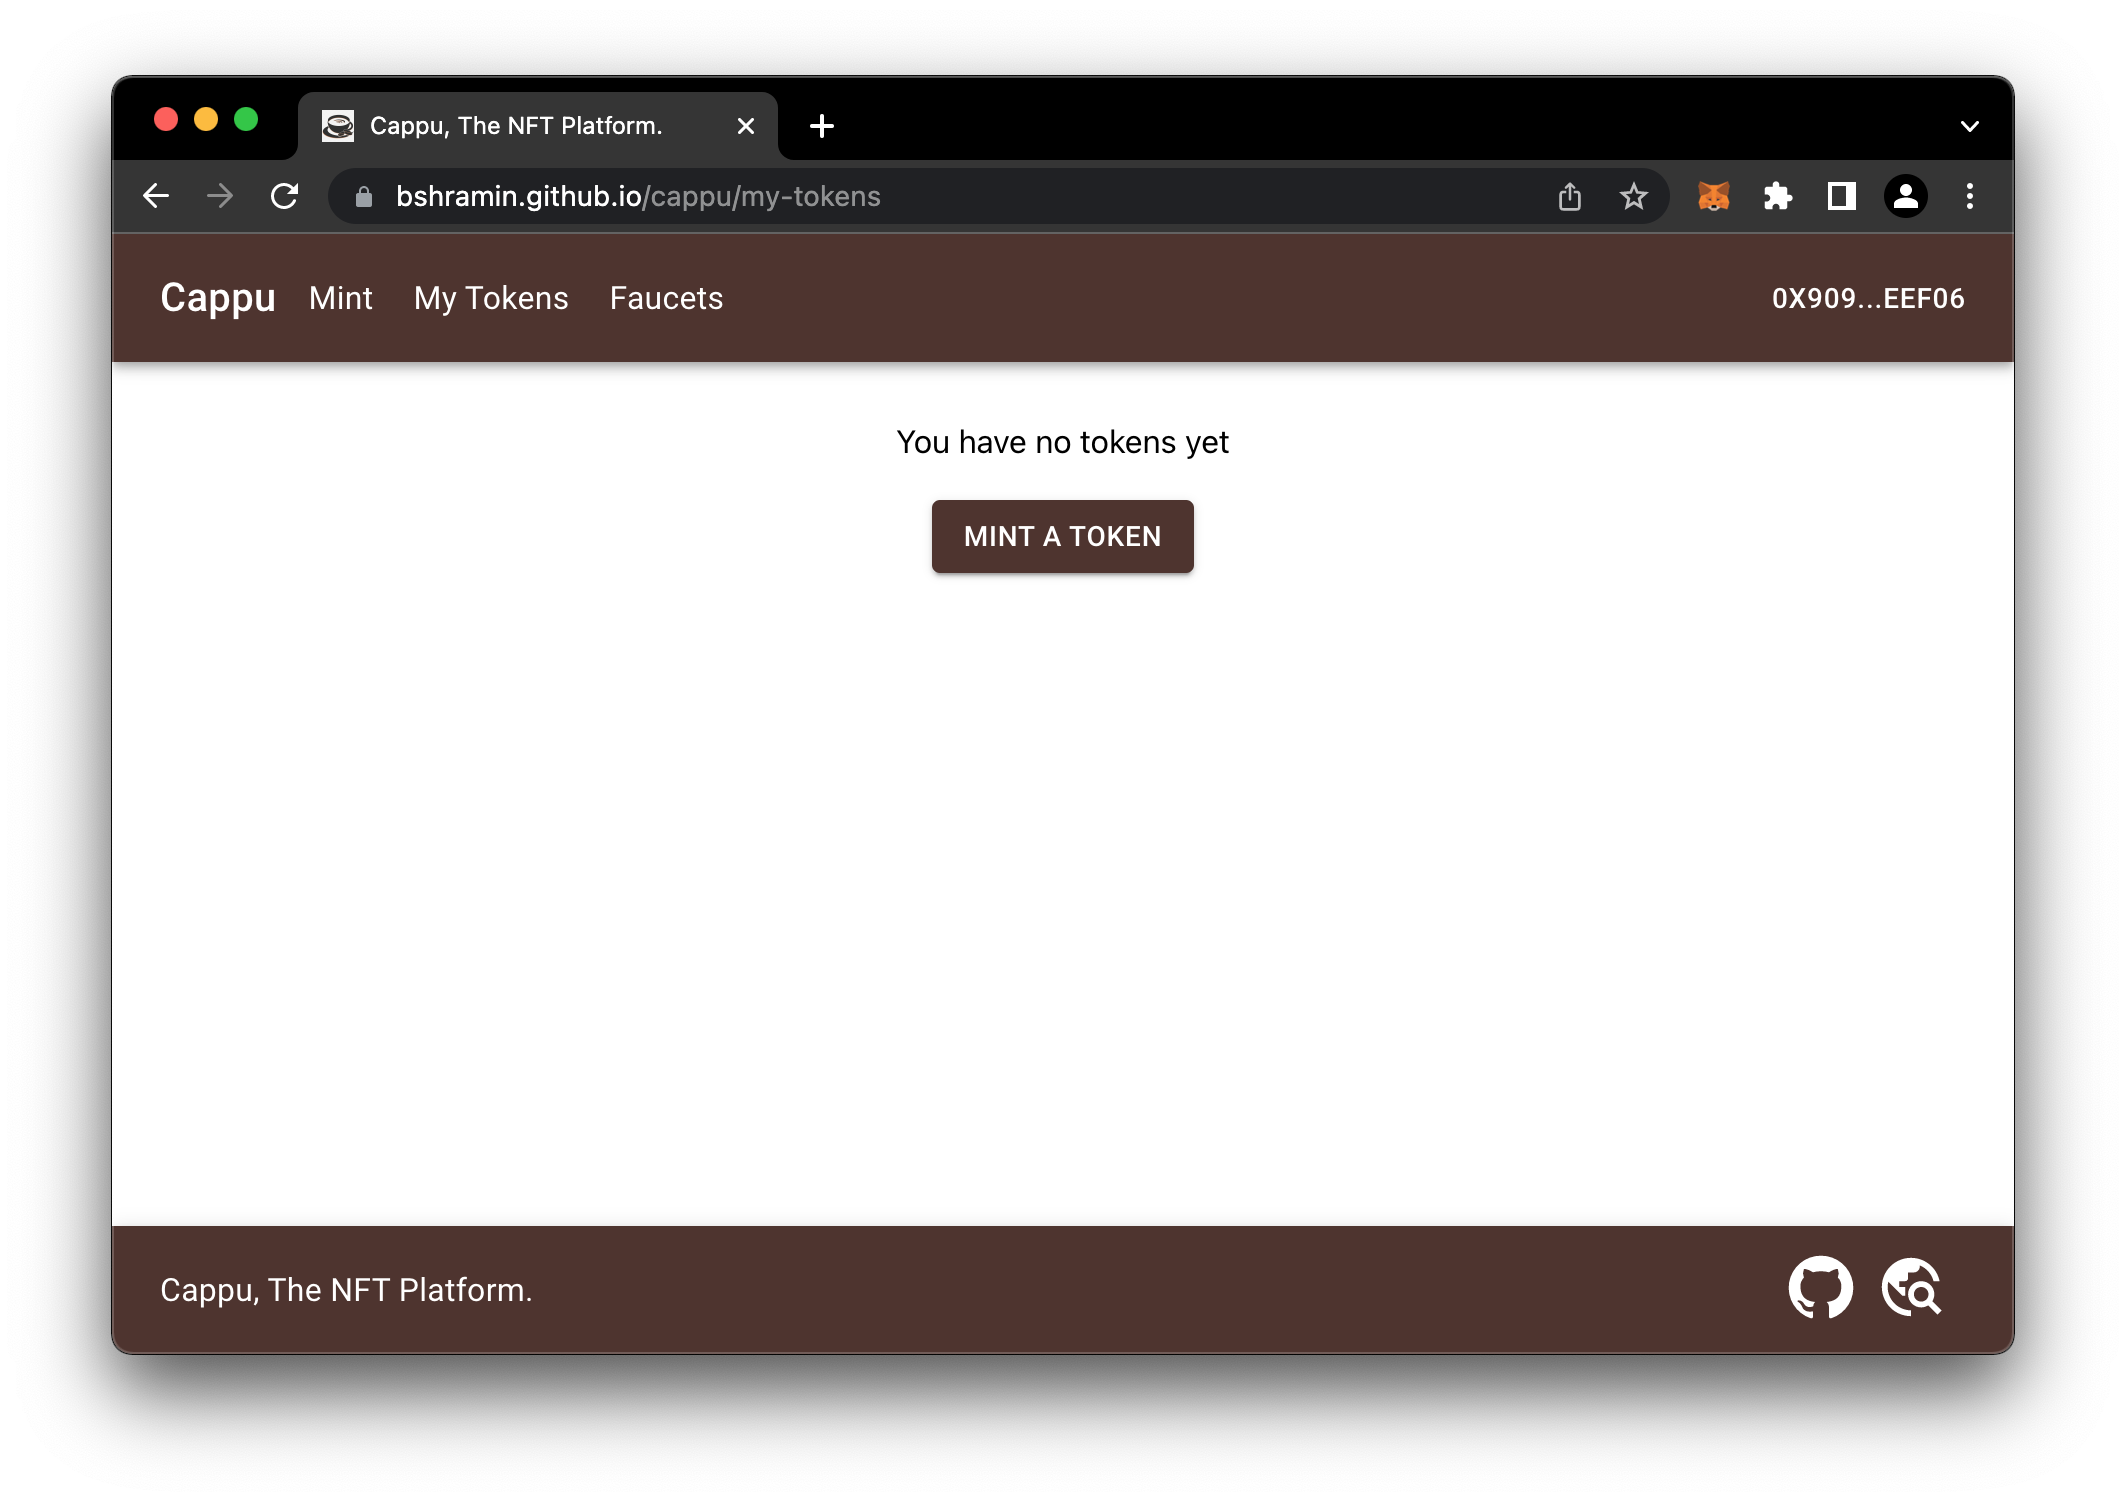
\includegraphics[width=12cm]{no-tokens-yet.png}}}
\caption{کاربر توکنی ندارد.}
\label{fig:no-tokens-yet}
\end{figure}

\begin{figure}
\centerline{\frame{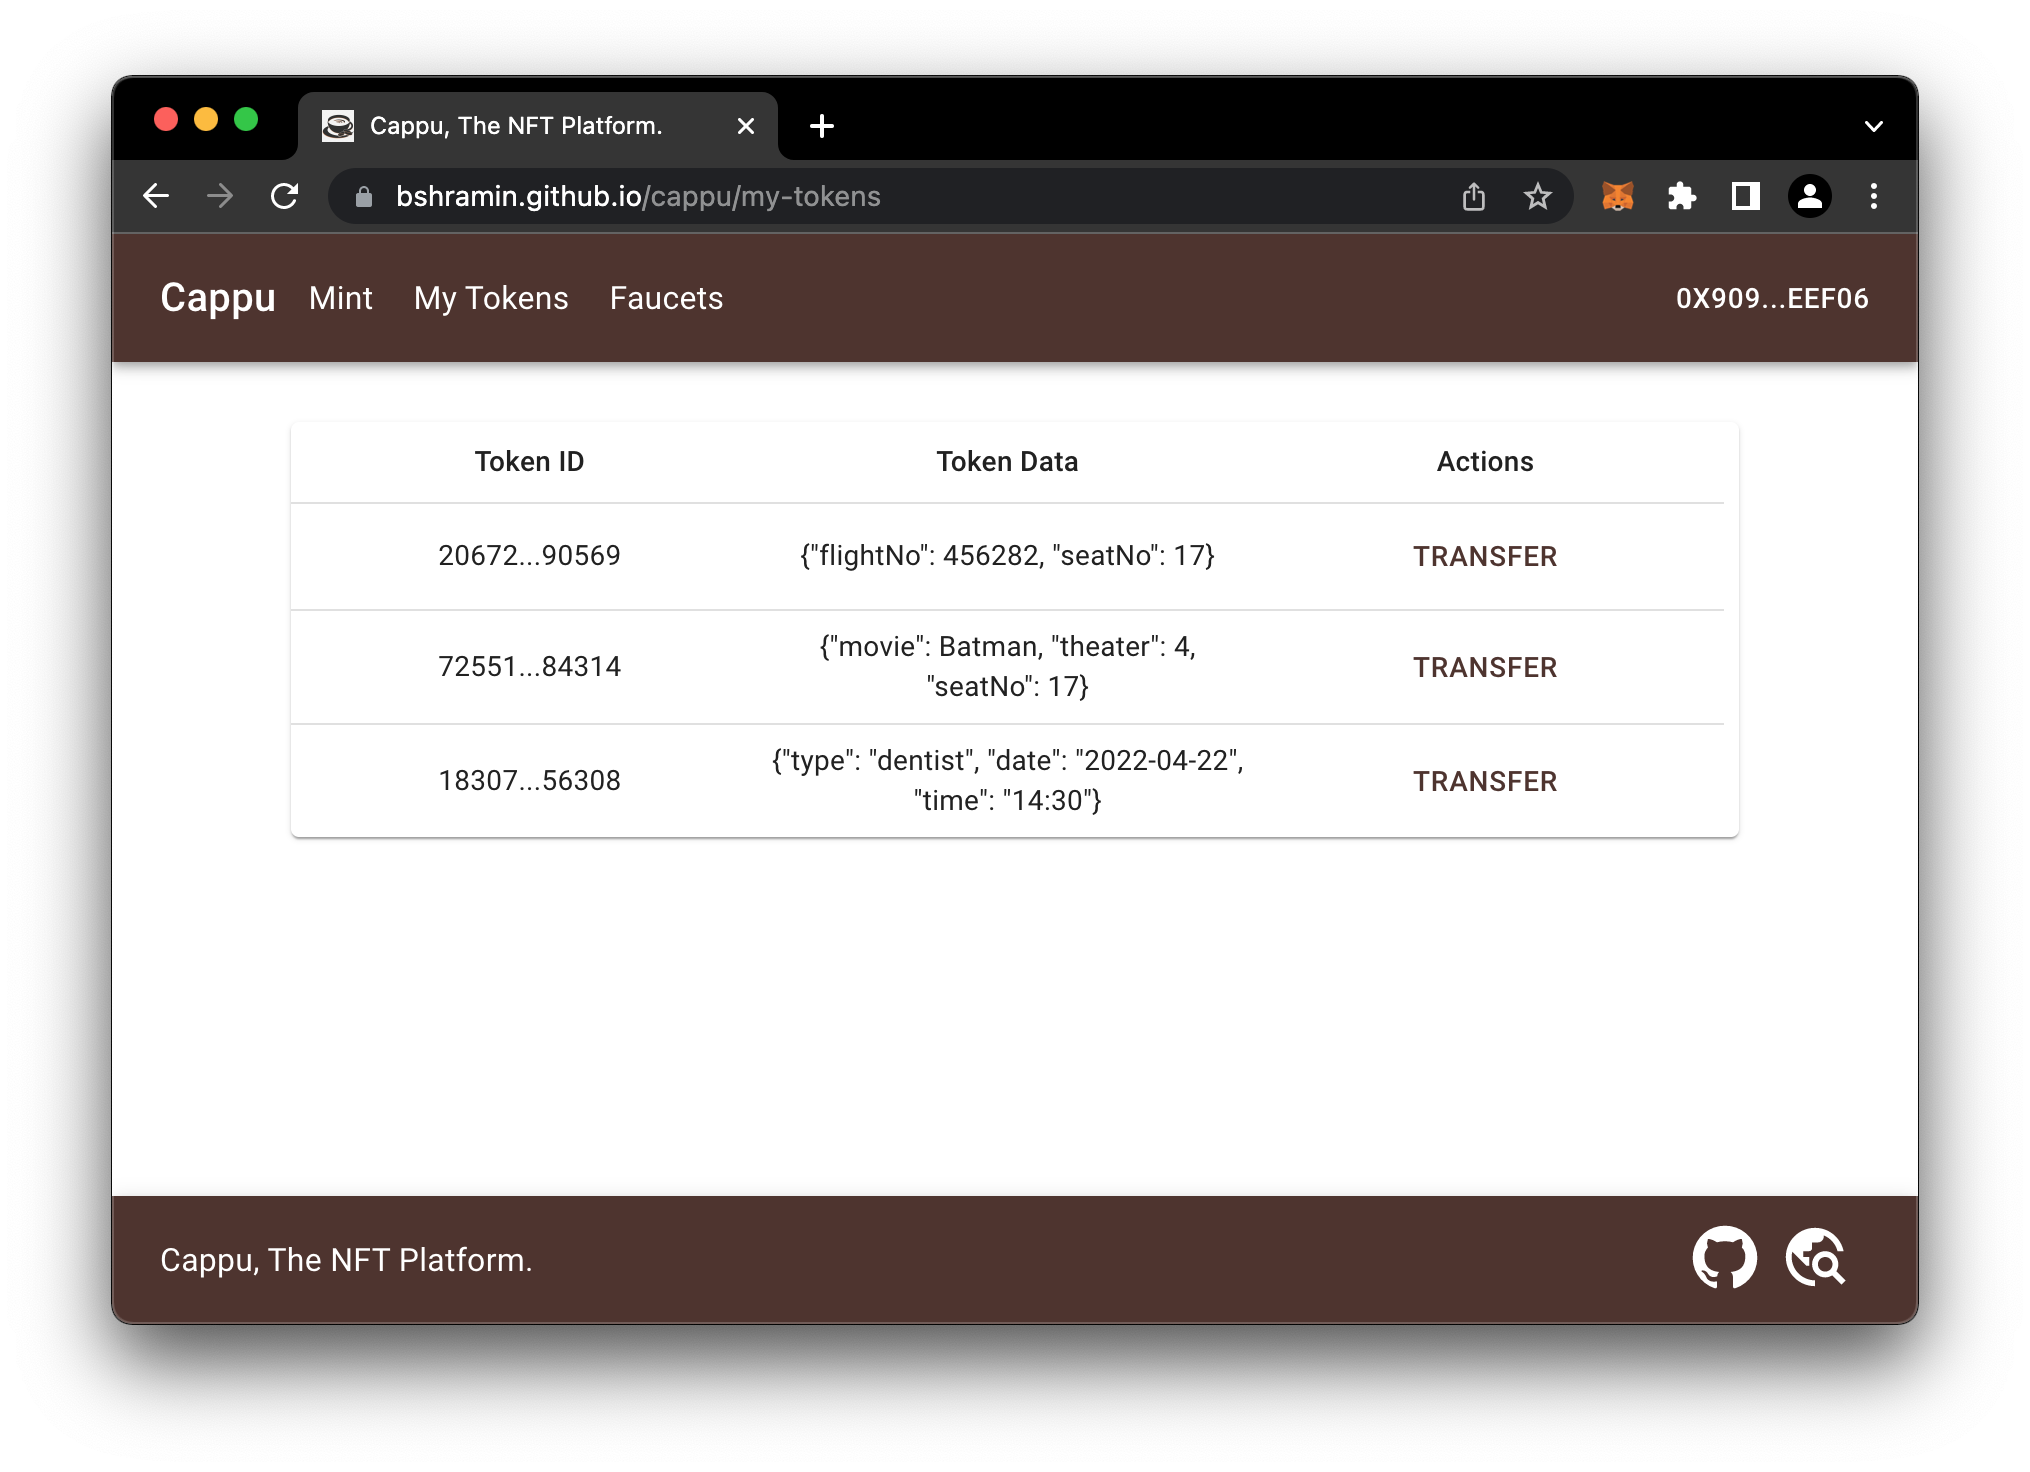
\includegraphics[width=12cm]{tokens-list.png}}}
\caption{لیست توکن‌های کاربر.}
\label{fig:tokens-list}
\end{figure}

در این صفحه کاربر می‌تواند هر یک از توکن‌ها را با انتخاب دکمه
\lr{Transfer}
به شخص دیگری ارسال کند.
با انتخاب گزینه انتقال توکن،
صفحه‌ی کوچکی مانند تصویر
\ref{fig:transfer-modal}
باز می‌شود که کاربر میتواند در آن آدرس مقصد را وارد کرده و توکن را ارسال کند.
پس از فشردن دکمه انتقال، مانند تصویر
\ref{fig:transfer-loading}
پیام انتظار به کاربر نمابش داده می‌شود.
در صورت موفق بودن انتقال کاربر مانند تصویر
\ref{fig:transfer-success}
پیام موفقیت را مشاهده می‌کند.
همچنین اگر تراکنش با مشکلی مواجه شود نیز پیام مناسب مانند تصویر
\ref{fig:transfer-error}
به کاربر نمایش داده می شود.

\begin{figure}[H]
\centerline{\frame{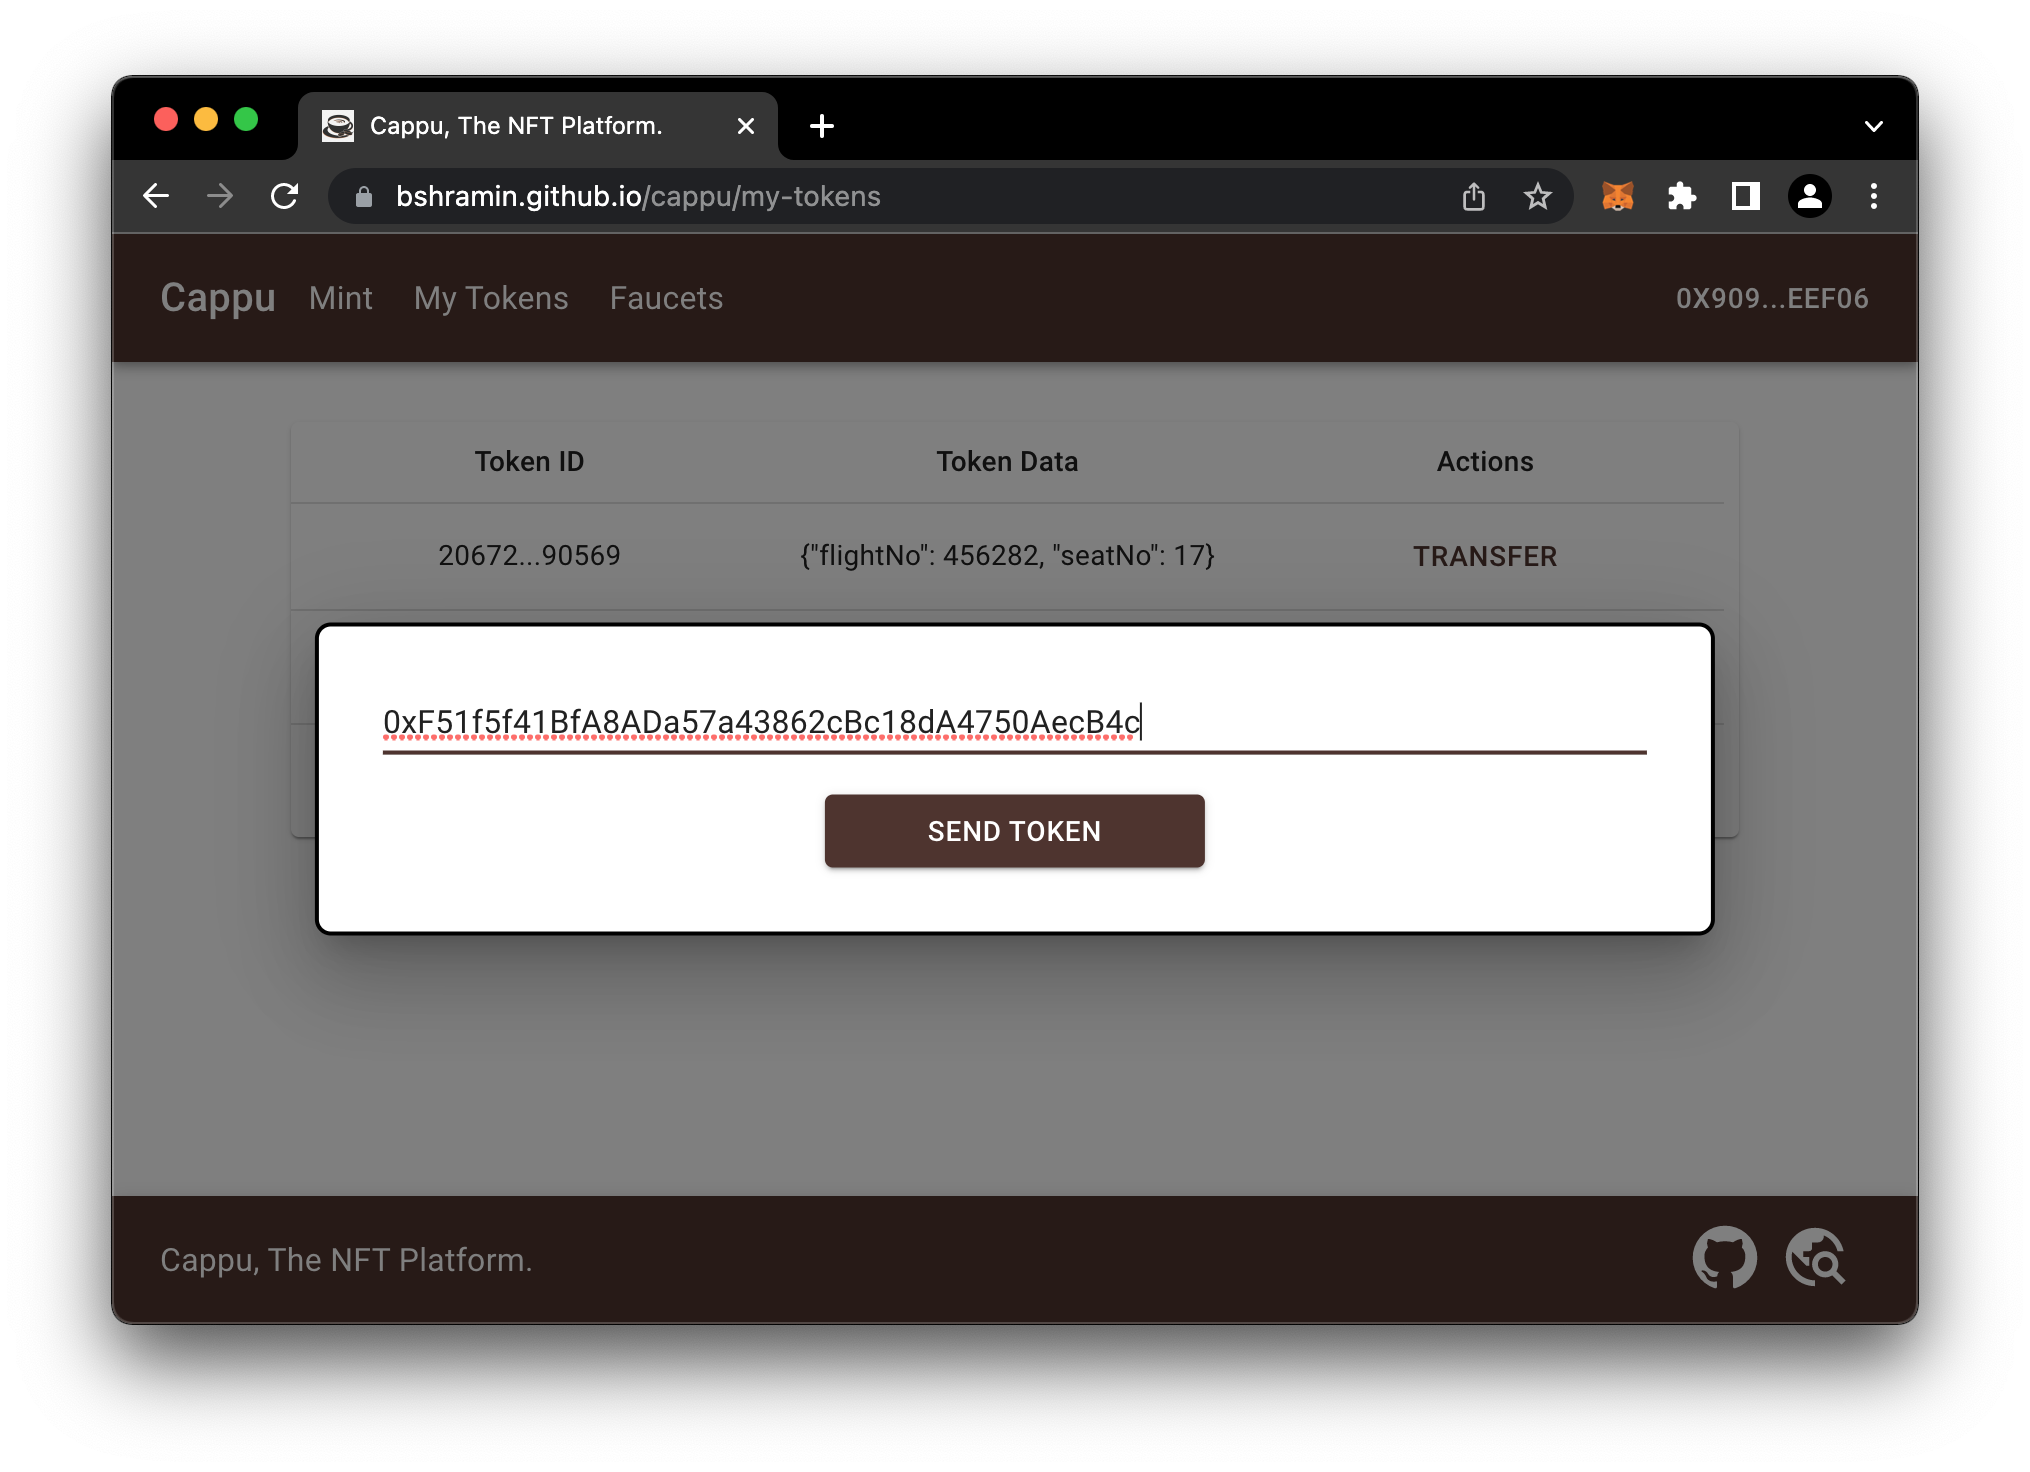
\includegraphics[width=12cm]{transfer-modal.png}}}
\caption{صفحه ورود آدرس مقصد و انتقال توکن.}
\label{fig:transfer-modal}
\end{figure}

\begin{figure}[H]
\centerline{\frame{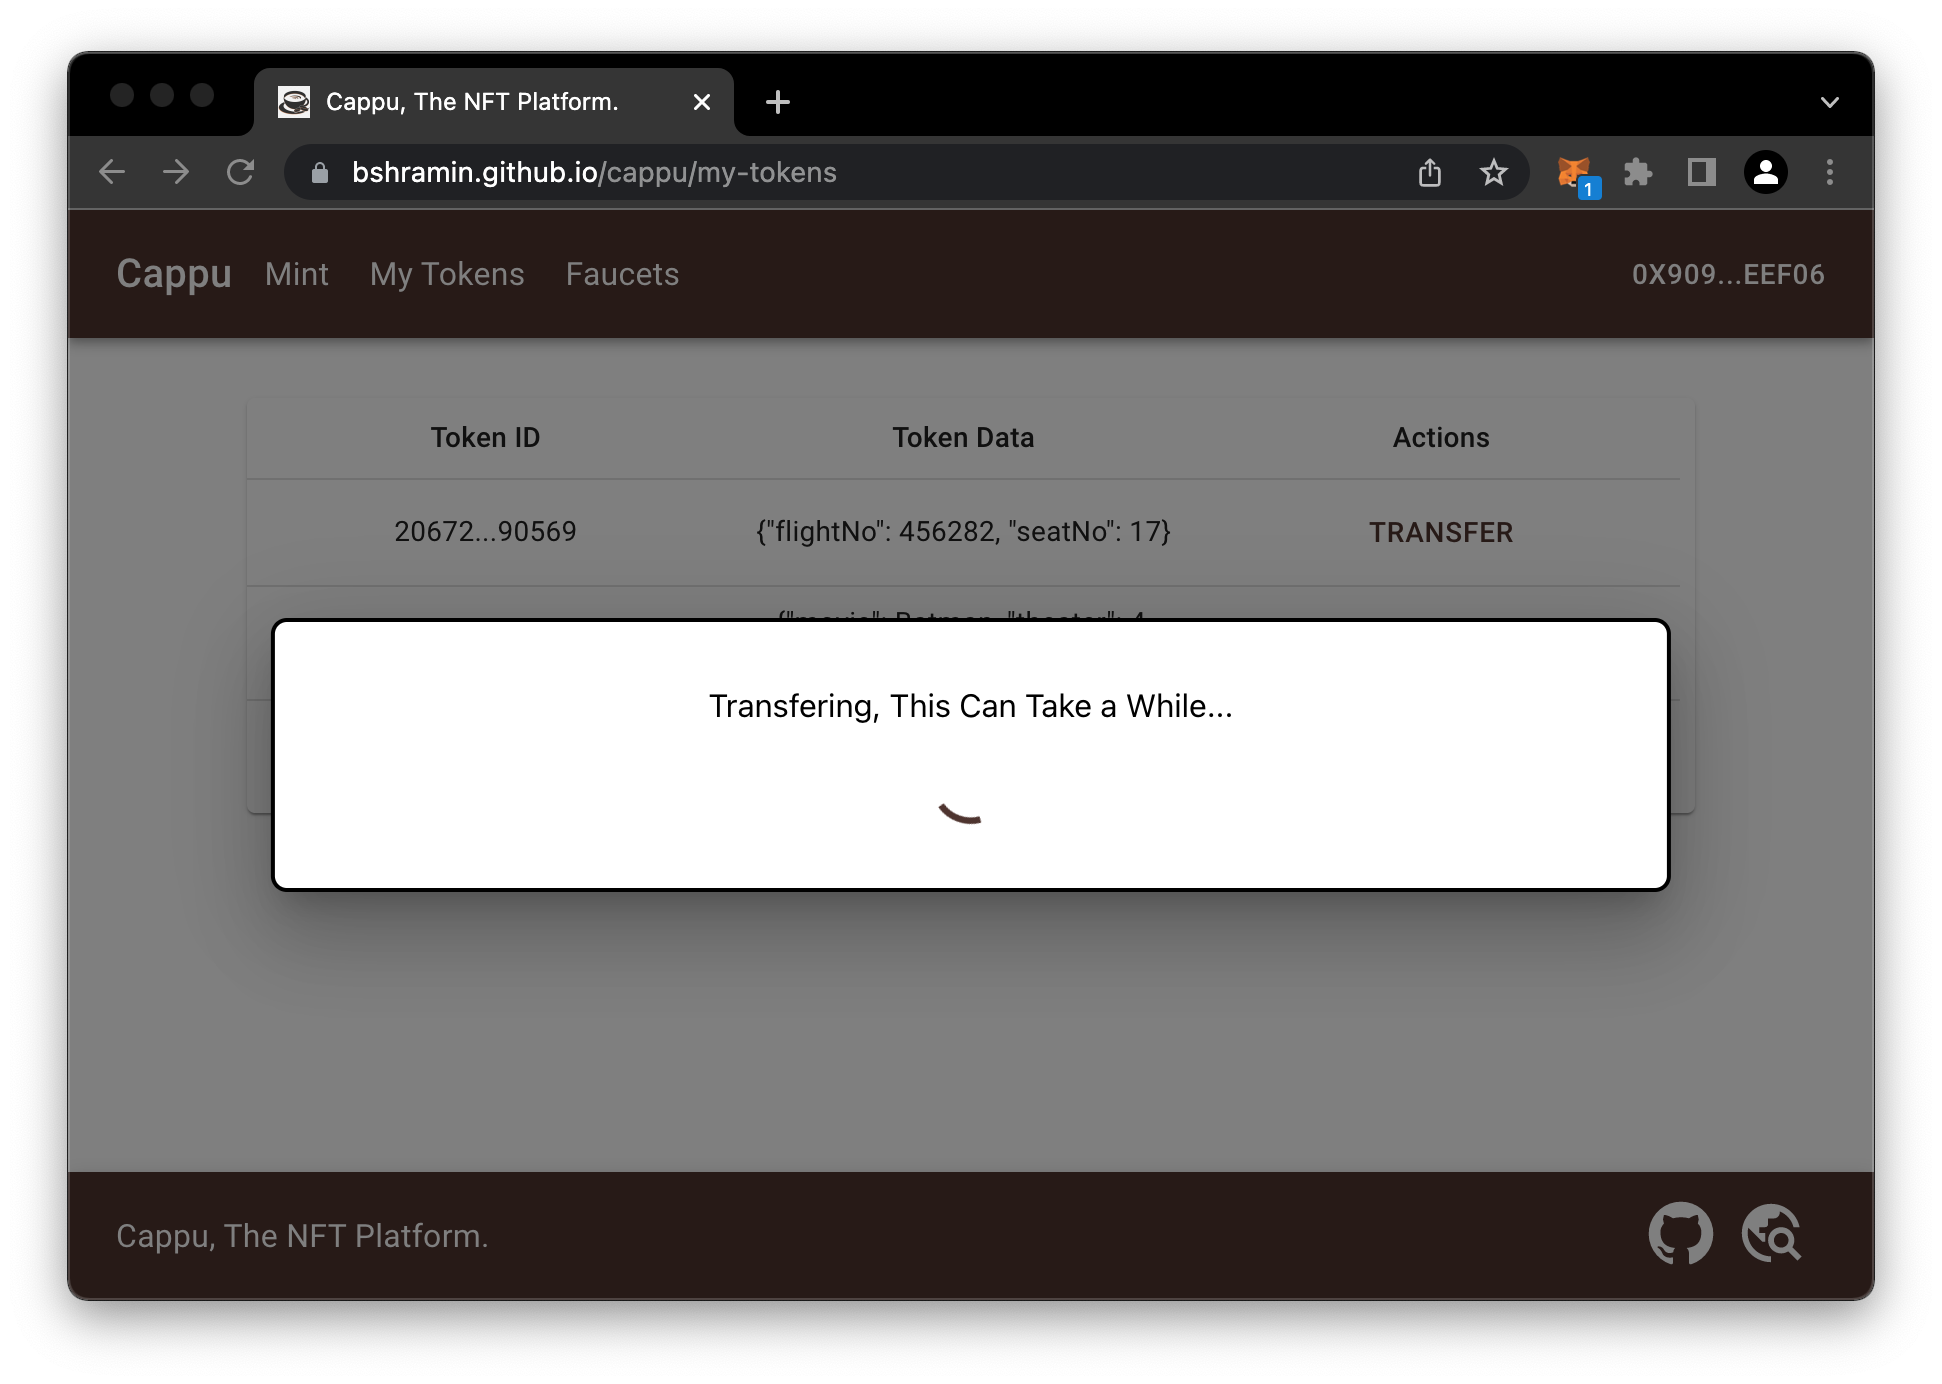
\includegraphics[width=12cm]{transfer-loading.png}}}
\caption{در حال ارسال توکن.}
\label{fig:transfer-loading}
\end{figure}

\begin{figure}[H]
\centerline{\frame{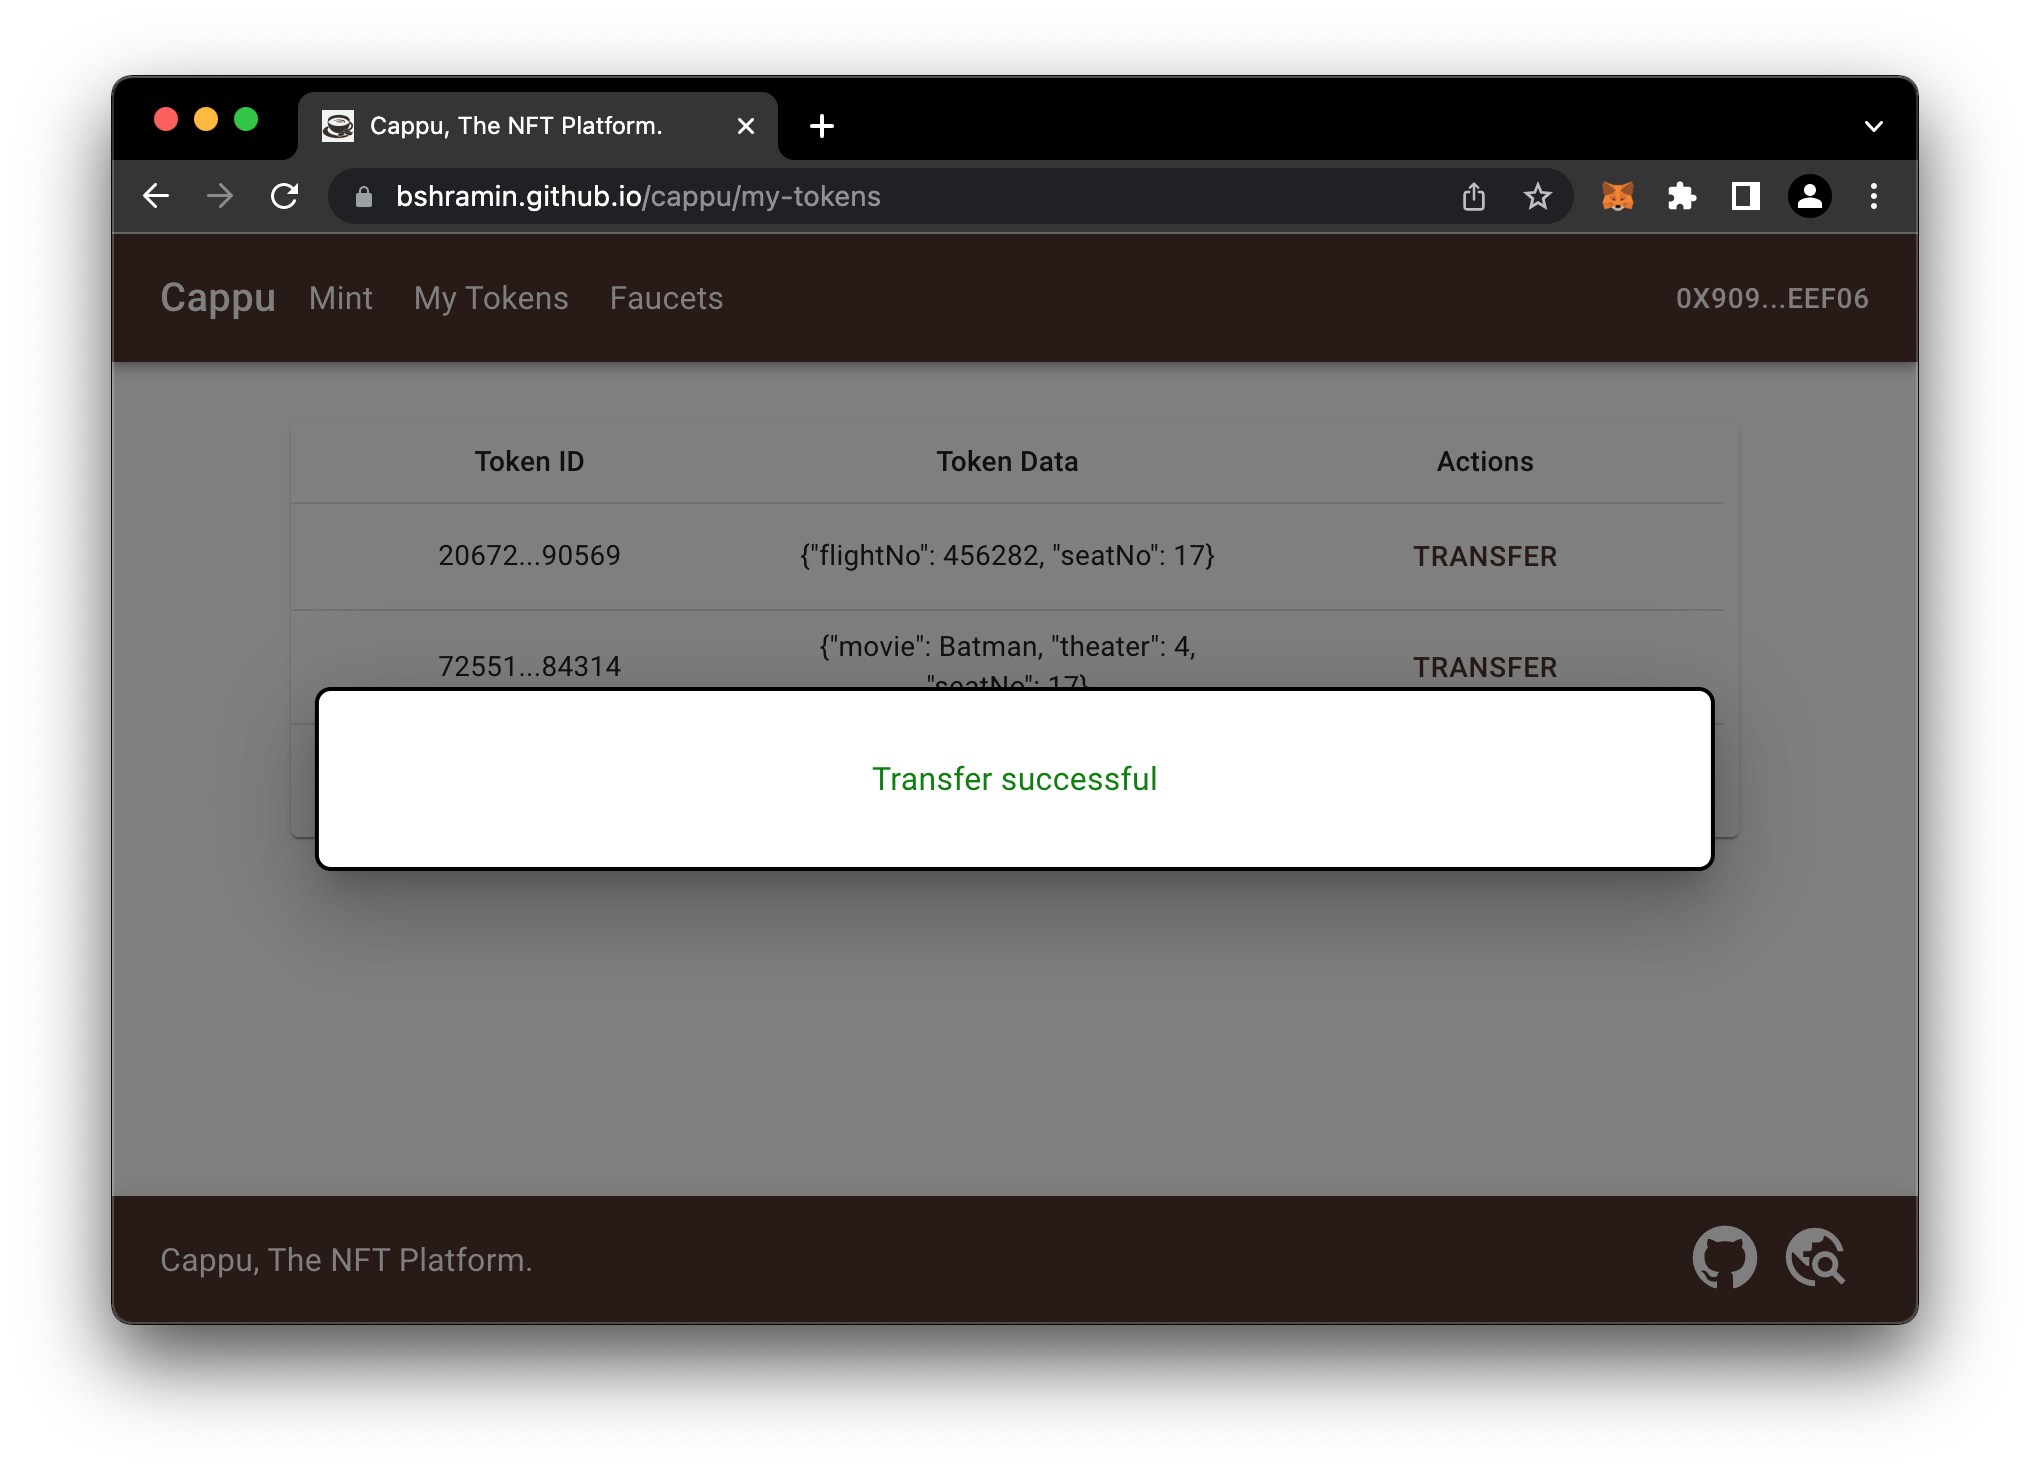
\includegraphics[width=12cm]{transfer-success.png}}}
\caption{ارسال موفق توکن.}
\label{fig:transfer-success}
\end{figure}

\begin{figure}[H]
\centerline{\frame{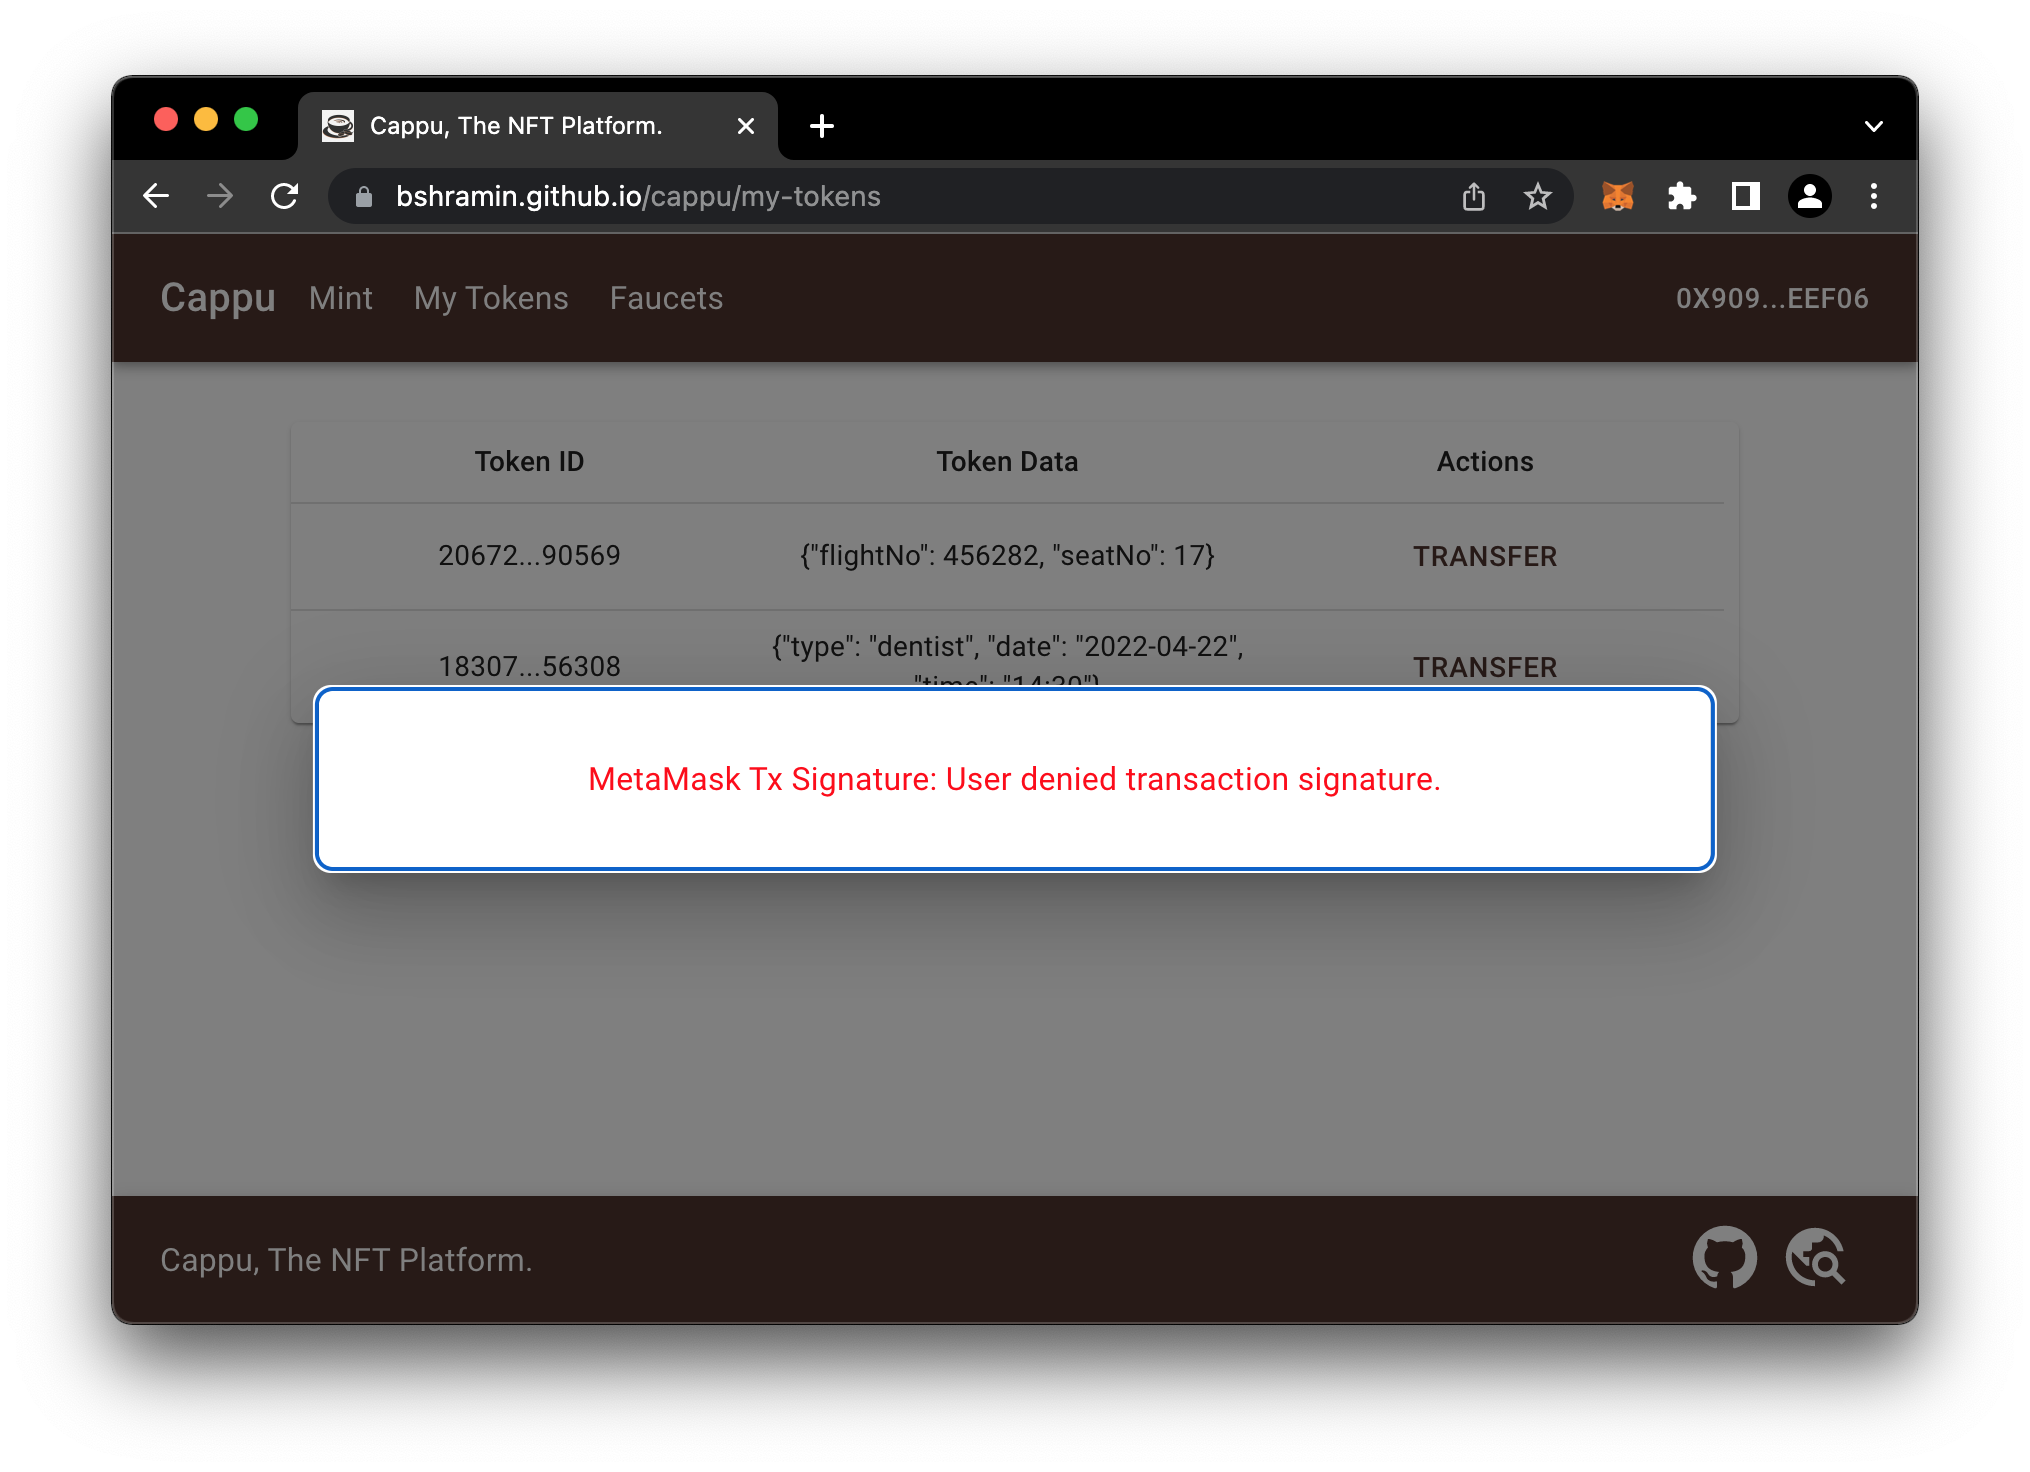
\includegraphics[width=12cm]{transfer-error.png}}}
\caption{ارسال توکن با مشکل مواجه شده.}
\label{fig:transfer-error}
\end{figure}















\subsection{بارگذاری واسط‌کاربری}
برای این که کاربرها بتوانند با قرارداد هوشمند ارتباط برقرار کنند نیاز است که واسط‌کاربری اپلیکیشن در سروری بارگذاری شود.
خوشبختانه گیت‌هاب قابلیت به نام
\gls{Github Pages}
در اختیار کاربرانش قرار می‌دهد
که به کمک آن می‌توان واسط‌کاربری اپلیکیشن را در آدرسی متناسب با آدرس مخزن کد در گیت‌هاب بارگذاری کرد
و کاربران با رجوع به آن آدرس می‌توانند واسط‌کاربری اپلیکیشن را ببینند و از آن استفاده کنند.

این قابلیت گیت‌هاب در واقع به این صورت عمل می‌کند که یک برنچ به نام
\lr{gh-pages}
در
\gls{Repository}
پروژه می‌سازد و هربار که دستور بارگذاری پروژه توسط گیت‌هاب اجرا می‌شود،
یک بیلد از پروژه می‌گیرد و فایل‌های خروجی بیلد روی این برنچ پوش می‌شوند.
سپس این فایل‌ها روی آدرسی متناسب با آدرس مخزن کد‌های پروژه بارگذاری می‌شوند.
برای مثال آدرس ریپازیتوری و واسط‌کاربری اپلیکیشن کاپو به صورت زیر است:
\begin{itemize}
  \item
  آدرس ریپازیتوری: \url{https://github.com/bshramin/cappu}
  \item
  آدرس واسط‌کاربری: \url{https://bshramin.github.io/cappu}
\end{itemize}
البته بارگذاری شدن واسط‌کاربری روی صفحات گیت‌هاب با ایجاد مشکلاتی در
\gls{Routing}
همراه بود که رفع شدند.


% ------------ Section 4.5
\section{داکرایز شدن، پایپلاین‌ها وگیت}
اقدامات زیر به منظور سرعت بخشیدن و تسهیل فرآیندهای توسعه و بارگذاری انجام شدند.

\subsection{داکرایز شدن تست‌های قرارداد هوشمند}
برای سرعت بخشیدن به توسعه قرارداد هوشمند،
این نیازمندی به وجود آمد که بعد از پوش شدن هر تغییر روی گیت‌هاب تست‌های قرارداد به صورت خودکار اجرا شوند.
به این منظور نیاز است که تست‌های قرارداد هوشمند بتوانند در یک کانتینر داکر اجرا شوند.

برای داکرایز کردن اجرای تست‌های قرارداد هوشمند،
نخست سعی در این بود که یک ایمیج داکر پایه که ترافل روی آن نصب شده باشد پیدا شود،
اما نسخه ترافل نمونه‌هایی که یافت شد با نسخه مورد نظر همخوانی نداشت.
در نتیجه یک ایمیج پایه داکر نوشته شد که داکرفایل آن را می‌توان در گیت‌هاب
\LTRfootnote{
  \url{https://github.com/bshramin/truffle-docker}
}
مشاهده کرد، همچنین این ایمیج داکر در داکرهاب
\LTRfootnote{
  \url{https://hub.docker.com/r/aminbshr/truffle}
}
نیز پوش شد.

سپس داکرفایل دیگری نوشته شد که با استفاده از این ایمیج پایه تست‌های قرارداد را اجرا کند.
تست‌های قرارداد در این ایمیج که ترافل بر روی آن نصب شده است با اجرای دستور
\lr{truffle test}
اجرا می‌شود.


\subsection{اجرای خودکار تست‌های قرارداد}
با داشتن داکرفایلی که با بیلد و اجرای آن تست‌های قرارداد هوشمند اجرا می‌شوند،
تست‌های قرارداد هوشمند می‌توانند به عنوان یکی از مراحل پایپلاین پروژه در گیت‌هاب نیز اجرا گردند.
به این صورت در هر مرج ریکوئست به
\gls{Master branch}
و با پوش شدن یک کامیت در برنچ اصلی تست‌ها به صورت خودکار در پایپلاین گیت‌هاب اجرا می‌شوند.
به این ترتیب سرعت توسعه و اطمینان از کدهای قرارداد بیشتر می‌شود.


\subsection{بارگذاری خودکار واسط‌کاربری}
برای ساده‌سازی بیشتر فرآیند بارگذاری واسط‌کاربری و سرعت بخشیدن به توسعه آن،
این قابلیت پیاده سازی می‌شود که پس از هربار ایجاد تغییر در واسط‌کاربری،
به جای این که توسعه‌دهنده با اجرای دستوراتی واسط‌کاربری را به کمک صفحات گیت‌هاب بارگذاری کند،
واسط‌کاربری پس از پوش شدن تغییرات جدید روی برنچ اصلی ریپازیتوری بارگذاری می‌شود.

برای پیاده‌سازی این قابلیت از
\lr{Github Actions}
که در واقع پایپلاین‌های گیت‌هاب برای یک پروژه هستند استفاده می‌شود.
تنها نکته‌ای که باید به آن توجه شود این است که این استیج از پایپلاین یک تفاوت اصلی با استیج‌های دیگر دارد.
استیج‌های دیگر فقط می‌خواهند که کدهای ریپازیتوری را بخوانند و نمی‌خواهند چیزی را در ریپازیتوری تغییر دهند،
اما این استیج می‌خواهد که کد‌های واسط‌کاربری را بیلد کند و سپس فایل‌های بیلد شده را روی برنچ دیگری به نام
\lr{gh-pages}
پوش کند. پس این استیج پایپلاین نیاز به دسترسی پوش کردن کد روی ریپازیتوری دارد.

برای پیاده‌سازی این قابلیت به این صورت عمل می‌شود که نخست یک داکرفایل نوشته می‌شود
که در آن کدهای واسط‌کاربری بیلد و سپس به کمک صفحات گیت‌هاب روی برنچ
\lr{gh-pages}
پوش و بارگذاری می‌شوند.
اما این کانتینر برای این که بتواند کدها را روی ریپازیتوری پوش کند نیاز به یک توکن از گیت‌هاب دارد،
به همین دلیل برای این داکرفایل یک
\gls{Environment variable}
تعریف می‌شود و هنگامی که در استیج بارگذاری واسط‌کاربری این داکرفایل بیلد
و اجرا می‌شود توکنی که از گیت‌هاب گرفته شده است به عنوان
\gls{Environment variable}
به این کانتینر داده می‌شود. به این ترتیب این توکن درون کانتینر داکر وجود خواهد داشت و
\lr{Github Pages}
از آن استفاده خواهد کرد.

